%%%%%
%%%%%  Naudokite LUALATEX, ne LATEX.
%%%%%
%%%%
\documentclass[]{VUMIFTemplateClass}

\usepackage{indentfirst}
\usepackage{amsmath, amsthm, amssymb, amsfonts}
\usepackage{mathtools}
\usepackage{physics}
\usepackage{graphicx}
\usepackage{verbatim}
\usepackage[hidelinks]{hyperref}
\usepackage{color,algorithm,algorithmic}
\usepackage[nottoc]{tocbibind}
\usepackage{tocloft}
\usepackage{booktabs}
\usepackage{array}
\usepackage{longtable}

\usepackage{titlesec}
\newcommand{\sectionbreak}{\clearpage}

\makeatletter
\renewcommand{\fnum@algorithm}{\thealgorithm}
\makeatother
\renewcommand\thealgorithm{\arabic{algorithm} algoritmas}

\usepackage{biblatex}
\bibliography{bibliografija}
%% Bibliografijos stilius nustatytas VUMIFTemplateClass.cls (style=ieee).

%% Lentelės antraštė: "lentelė N. <tekstas>" (vietoj polyglossia numatyto "N lentelė.")
\makeatletter
\AtBeginDocument{\def\fnum@table{\tablename\nobreakspace\thetable}}
\makeatother

% Author's MACROS
\newcommand{\EE}{\mathbb{E}\,}
\newcommand{\ee}{{\mathrm e}}
\newcommand{\RR}{\mathbb{R}}


\studijuprograma{Informacinių sistemų inžinerijos} % kilmininko linksniu, nes titulinis.tex prijungia "studijų programa"
\darbotipas{Trečiasis laboratorinis darbas}
\darbopavadinimas{Vaizdų ir laiko eilučių klasifikavimas naudojant konvoliucinius neuroninius tinklus}
\autorius{Matas Semėnas}

\vadovas{Viktor Medvedev, Doc., Dr.}

\begin{document}
\selectlanguage{lithuanian}

\onehalfspacing
\input{titulinis}

\selectlanguage{lithuanian}

\singlespacing

%Turinys
\tableofcontents
\onehalfspacing


%Sutrumpinimų skyrius
% \sectionnonum{Santrumpos}
% Šiame skyrelyje pateikiamos darbe naudojamos santrumpos.

% \begin{tabular}{rcp{.7\textwidth}}
%     {KNT}  & {--} & {konvoliucinis neuroninis tinklas (angl.\ \textit{convolutional neural network})}\\
%     {CNN}  & {--} & {\textit{convolutional neural network}}\\
%     {2D}   & {--} & {dvimatis (angl.\ \textit{two-dimensional})}\\
%     {1D}   & {--} & {vienmatis (angl.\ \textit{one-dimensional})}\\
%     {BN}   & {--} & {paketų normalizavimas (angl.\ \textit{batch normalization})}\\
%     {ReLU} & {--} & {ištaisyto tiesinio vieneto aktyvacija (angl.\ \textit{rectified linear unit})}\\
%     {RPS}  & {--} & {„Akmuo--popierius--žirklės“ duomenų rinkinys (angl.\ \textit{rock-paper-scissors})}\\
%     {CMU}  & {--} & {Carnegie Mellon universitetas (angl.\ \textit{Carnegie Mellon University})}\\
%     {CPU}  & {--} & {centrinis procesorius}\\
%     {GPU}  & {--} & {grafinis procesorius}\\
% \end{tabular}


\sectionnonum{Darbo tikslas}

Šio laboratorinio darbo tikslas --- pritaikyti konvoliucinio neuroninio tiklo modelį (toliau --- CNN) klasifikuoti vaizdams ir laiko eilutei bei įvertinti, atlikti tyrimą kaip galutinį klasifikavimo tikslumą įtakoja tinklo architektūra ir pagrindiniai hiperparametrai (išmetimo (\textit{dropout}) tikimybė, paketų normalizavimas, aktyvacijos funkcija, optimizavimo algoritmas).


\section{Duomenys}\label{sec:duomenys}

\subsection{Vaizdų duomenų rinkinys}

Vaizdų klasifikavimo užduočiai pasirinktas  „Akmuo--popierius--žirklės“ duomenų rinkinys iš \textit{Kaggle} platformos~\cite{rps_dataset}. Duomenų rinkinį sudaro spalvotos rankos gestų nuotraukos vienodame žaliame fone, sugrupuotos į tris klases: \texttt{paper} (popierius), \texttt{rock} (akmuo) ir \texttt{scissors} (žirklės). Nuotraukų rezoliucija --- \(300{\times}200\) pikselių, RGB.

Klasių dažnio pasiskirstymas pateiktas lentelėje~\ref{tab:rps_kiekiai}. Duomenų rinkinyje yra 2188 nuotraukos, klasės subalansuotos (didžiausias skirtumas tarp klasių --- \(\sim 5{,}3~\%\)), todėl papildomas klasių balansavimas netaikomas.

\begin{table}[H]
    \centering
    \caption{Vaizdų rinkinio klasių dažniai}
    \label{tab:rps_kiekiai}
    \begin{tabular}{|l|c|}
        \hline
        \textbf{Klasė} & \textbf{Vaizdų skaičius}\\
        \hline
        \texttt{paper} (popierius)   & 712 \\
        \hline
        \texttt{rock} (akmuo)        & 726 \\
        \hline
        \texttt{scissors} (žirklės)  & 750 \\
        \hline
        \textbf{Iš viso}             & \textbf{2188} \\
        \hline
    \end{tabular}
\end{table}

\subsection{Laiko eilučių duomenų rinkinys}

Laiko eilučių klasifikavimo eksperimentui naudojama Carnegie Mellon universiteto klavišų paspaudimų dinamikos duomenų aibė~\cite{cmu_keystroke}. Visi dalyviai, 8 atskirų sesijų metu po 50 kartų iš naujo įvedė vienodą fiksuotą slaptažodį \texttt{tie5Roanl}. Duomenyse randami trijų rūšių laikai:
\begin{itemize}
    \item \textit{H} (\textit{hold}) --- klavišo paspaudimo trukmė;
    \item \textit{DD} (\textit{down-down}) --- laikas tarp dviejų gretimų klavišų paspaudimų;
    \item \textit{UD} (\textit{up-down}) --- laikas nuo ankstesnio klavišo atleidimo iki kito klavišo paspaudimo.
\end{itemize}

Gaunama 31 skaitinių požymių laiko eilutė vienam slaptažodžio surinkimui. Pagal užduoties reikalavimą atrinkti pirmieji 30 dalyvių (rūšiuojant abėcėliškai pagal subjekto identifikatorių) ir naudojama tik viena sesija (\(\texttt{sessionIndex} = 1\)). Kiekvienas dalyvis sesijoje atliko 50 surinkimų, todėl iš viso turima \(30 \times 50 = 1500\) įrašų. Kiekvienam dalyvis turi 50 įrašų vienoje klasėje, todėl duomenys yra tobulai subalansuoti.


\section{Duomenų paruošimas}\label{sec:paruosimas}

Abiem duomenų rinkiniams taikomas tas pats \(80:10:10\) sąntykio padalinimas, kuris realizuotas dviem \texttt{train\_test\_split} kvietimais (pirmas atskiria 20~\% duomenų, antras juos padalina į validavimo ir testavimo aibes po lygiai). Užtikrinama, kad kiekviena aibė išlaikytų panašią klasių proporciją kaip ir originalus rinkinys. Visiems atsitiktinumo šaltiniams (\texttt{random}, \texttt{numpy}, \texttt{tensorflow}) nustatytas vienodas \(\texttt{SEED} = 42\), todėl rezultatai yra atkuriami.

Duomenų aibių dydžiai pateikti lentelėje~\ref{tab:splits}.

\begin{table}[H]
    \centering
    \caption{Duomenų rinkinių padalinimo rezultatai}
    \label{tab:splits}
    \begin{tabular}{|l|c|c|c|c|}
        \hline
        \textbf{Rinkinys} & \textbf{Mokymo aibė} & \textbf{Validavimo aibė} & \textbf{Testavimo aibė} & \textbf{Iš viso}\\
        \hline
        Vaizdai    & 1750 & 219 & 219 & 2188 \\
        \hline
        Laiko eilutės & 1200 & 150  & 150  & 1500 \\
        \hline
    \end{tabular}
\end{table}

\subsection{Vaizdų paruošimas}

Vaizdai į atmintį įkraunami funkcija \texttt{tf.keras.utils.load\_img}, kuri kiekvieną vaizdą sumažina iki vienodos rezoliucijos \(128 \times 128\) pikselių. Originali \(300 \times 200\) raiška buvo sumažinta dėl dviejų priežasčių: modelių mokymas vyksta naudojant procesorių (toliau --- CPU), todėl reikia riboti atminties ir laiko sąnaudas; gestų atpažinimui užtenka mažesnės raiškos, klasės skiriasi pagal aiškiai atpažįstamas formas, ne smulkias detales. Pikselių reikšmės normalizuojamos į intervalą \([0; 1]\) padalinant iš \(255\), todėl CNN modelio įvestis yra (\texttt{float32}) tensorius (4D masyvas).

Visi vaizdai apjungiami į keturmačio masyvo formatą \((N, 128, 128, 3)\), tinkamą \texttt{Conv2D} sluoksniui.

\begin{verbatim}
X = np.asarray(X, dtype=np.float32)
y = np.asarray(y, dtype=np.int64)
\end{verbatim}

\subsection{Laiko eilučių paruošimas}

Duomenys įkraunami iš CSV failo (\texttt{pandas.read\_csv}). Atfiltruojami pirmieji 30 dalyvių ir tik pirmoji sesija. Duomenys saugomi dvimačio masyvo pavidalu \((N, 31)\), kuriame eilutė atitinka vieną slaptažodžio surinkimą.

\texttt{Conv1D} sluoksniui reikia \((N, L, C)\) tensoriaus formato, kur \(L\) --- sekos ilgis, o \(C\) --- kanalų skaičius, todėl pridedama tuščia kanalų ašis (\texttt{X[..., np.newaxis]}). Galutinė įvesties forma --- \((N, 31, 1)\). Kadangi skirtingi laiko požymiai turi skirtingą skalę, atliekamas standartizavimas (vidurkis 0, standartinis nuokrypis 1). Standartizavimo statistikos (\(\mu, \sigma\)) skaičiuojamos tik iš mokymo aibės ir tada taikomos validavimo bei testavimo aibėms.

\begin{verbatim}
mean = X_tr.mean(axis=(0, 2), keepdims=True)
std  = X_tr.std(axis=(0, 2), keepdims=True) + 1e-8
X_tr = (X_tr - mean) / std
X_va = (X_va - mean) / std
X_te = (X_te - mean) / std
\end{verbatim}


\section{Skaičiavimo resursai}\label{sec:resursai}

Visi eksperimentai atlikti asmeniniame nešiojamajame kompiuteryje, naudojant tik CPU. Pagrindinės specifikacijos pateiktos lentelėje~\ref{tab:hw}.

\begin{table}[H]
    \centering
    \caption{Naudoto kompiuterio aparatūros charakteristikos}
    \label{tab:hw}
    \begin{tabular}{|l|l|}
        \hline
        \textbf{Komponentas} & \textbf{Specifikacija}\\
        \hline
        Centrinis procesorius (CPU) & Intel Core i7-11800H (8 fiziniai / 16 loginiai branduoliai, iki 4{,}6 GHz)\\
        \hline
        Operatyvioji atmintis (RAM) & 16 GB DDR4\\
        \hline
        Operacinė sistema           & Linux (WSL po Windows 11)\\
        \hline
        Programinė aplinka          & Python 3.12, TensorFlow 2.21, Keras 3.12\\
        \hline
    \end{tabular}
\end{table}

Kadangi GPU nenaudojamas, atminties ir laiko sąnaudos buvo apribotos pasirenkant santykinai mažą vaizdo raišką (\(128 \times 128\)) bei vidutinį epochų skaičių (\(20\) vaizdams ir \(40\)--\(50\) laiko eilutėms). Visi 18 eksperimentų vienai duomenų aibei užtruko apie 30--40 minučių.


\section{Naudojami konvoliuciniai neuroniniai tinklai}\label{sec:tinklas}

\subsection{Bendra architektūros schema}

Visi šiame darbe naudojami modeliai sukurti \texttt{Keras}~\cite{keras_docs} \texttt{Sequential} API ir turi tą pačią parametrizuojamą struktūrą. Tinklą sudaro vienas ar keli konvoliucinių blokų sluoksniai ir paskui einanti tankiai sujungtų sluoksnių pakopa.

Parametrizuotas modelio implementavimas leidžia lengvai keisti tinklo gylį, branduolio dydį, filtrų skaičių, dropout tikimybę ir kitus dydžius.

\subsection{Hiperparametrų ribos}

Eksperimentų metu varijuoti dydžiai pateikiami lentelėje~\ref{tab:hp}.

\begin{table}[H]
    \centering
    \caption{Eksperimentuose tirtų hiperparametrų reikšmės}
    \label{tab:hp}
    \begin{tabular}{|l|l|l|}
        \hline
        \textbf{Hiperparametras} & \textbf{Vaizdai} & \textbf{Laiko eilutės}\\
        \hline
        Epochų skaičius & 20 & 40--50 \\ \hline
        Paketo dydis (\textit{batch}) & 32 & 32 \\ \hline
        Mokymosi greitis & 0{,}001 & 0{,}001 \\ \hline
        Branduolio (\textit{kernel}) dydis & 3 & 3 arba 5 \\ \hline
        \textit{Pooling} dydis & 2 & 2 (paskutiniame bloke 1) \\ \hline
        Dropout (\(p\)) & \(\{0{,}0;\ 0{,}25;\ 0{,}5\}\) & \(\{0{,}0;\ 0{,}25;\ 0{,}5\}\) \\ \hline
        Paketų normalizavimas & išjungtas/įjungtas & išjungtas/įjungtas \\ \hline
        Aktyvacijos funkcija & ReLU, tanh, ELU, Leaky ReLU & ReLU, tanh, ELU, Leaky ReLU \\ \hline
        Optimizatorius & Adam, SGD, RMSprop, AdamW & Adam, SGD, RMSprop, AdamW \\ \hline
        Nuostolių funkcija & \texttt{sparse\_categorical\_crossentropy} & \texttt{sparse\_categorical\_crossentropy} \\ \hline
    \end{tabular}
\end{table}

Pasirinkta nuostolių funkcija \texttt{sparse\_categorical\_crossentropy}. Tai klasikinis daugiaklasės klasifikacijos pasirinkimas. \texttt{ChatGPT}.

\subsection{Tirtos architektūros}

Lyginamos trys skirtingo gylio architektūros (žr. lentelę~\ref{tab:archs}). Kiekviena turi vis daugiau konvoliucinių blokų ir tankių sluoksnių; Hipotezė --- gilesnis tinklas geriau atspindi sudėtingesnius požymius, bet rizikuoja persimokyti.

\begin{table}[H]
    \centering
    \caption{Lygintos CNN architektūros}
    \label{tab:archs}
    \begin{tabular}{|l|l|l|}
        \hline
        \textbf{Pavadinimas} & \textbf{Konvoliuciniai filtrai per blokus} & \textbf{Tankūs sluoksniai}\\
        \hline
        \texttt{arch\_small}  & 32, 64                  & 64        \\
        \hline
        \texttt{arch\_medium} & 32, 64, 128             & 128       \\
        \hline
        \texttt{arch\_large}  & 32, 64, 128, 128 (vaizdams) / 64, 128, 128, 64 (laiko eil.) & 256, 128 \\
        \hline
    \end{tabular}
\end{table}

Laiko eilučių atveju, paskutiniame konvoliuciniame bloke \texttt{pool=1} (pooling sluoksnis praleidžiamas), nes pradinis sekos ilgis tik 31 ir keturi \texttt{pool=2} sluoksniai sunaikintų laiko struktūrą.


\section{Programinis kodas}\label{sec:kodas}

\subsection{Naudoti įrankiai ir bibliotekos}

Programinis kodas parašytas Python programavimo kalba. Pagrindinės bibliotekos pateiktos lentelėje~\ref{tab:libs}.

\begin{table}[H]
    \centering
    \caption{Naudotos Python bibliotekos ir jų versijos}
    \label{tab:libs}
    \begin{tabular}{|l|l|l|}
        \hline
        \textbf{Biblioteka} & \textbf{Versija} & \textbf{Paskirtis}\\
        \hline
        TensorFlow~\cite{tensorflow}   & 2.21.0  & gilaus mokymosi karkasas\\
        Keras~\cite{keras_docs}        & 3.12.1  & aukšto lygio neuroninių tinklų API\\
        scikit-learn~\cite{sklearn}    & 1.7.2   & duomenų padalinimas, \texttt{confusion matrix}\\
        NumPy                          & 2.2.6   & skaitmeninių masyvų operacijos\\
        Pandas                         & 2.3.3   & CSV nuskaitymas\\
        Matplotlib                     & 3.10.8  & grafinės iliustracijos\\
        \hline
    \end{tabular}
\end{table}

Programa suskirstyta į du modulius: \texttt{main.py} vaizdų klasifikavimui (Conv2D), \texttt{main\_ts.py} laiko eilutėms (Conv1D). Abiejų modulių pagrindinė struktūra identiška: duomenų įkrovimas -- 80:10:10 padalinimas -- modelio kūrimo funkcija -- eksperimentai -- rezultatų išsaugojimas (\texttt{summary.csv}, mokymo kreivių grafikai, \texttt{confusion matrix} geriausiajam modeliui).

\subsection{Modelio konstravimas pagal konfigūraciją}

Funkcija \texttt{build\_model} paima \texttt{cfg} nustatymų rinkinį, kuris aprašo blokų sąrašą, tankius sluoksnius, optimizatorių, dropout tikimybes ir kt. Tai leidžia tarp eksperimentų keisti tinklo struktūrą. Sutrumpintas pavyzdys:

\begin{verbatim}
def build_model(cfg, input_shape, num_classes):
    model = models.Sequential(name=cfg["name"].replace(".", "_"))
    model.add(layers.Input(shape=input_shape))
    for i, blk in enumerate(cfg["blocks"]):
        use_bias = not blk.get("batch_norm", False)
        model.add(layers.Conv2D(blk["filters"], blk["kernel"],
                                padding="same", use_bias=use_bias))
        if blk.get("batch_norm", False):
            model.add(layers.BatchNormalization())
        model.add(make_activation_layer(blk["activation"]))
        if blk.get("pool", 0):
            model.add(layers.MaxPooling2D(pool_size=blk["pool"]))
        if blk.get("dropout", 0.0) > 0.0:
            model.add(layers.Dropout(blk["dropout"]))
    model.add(layers.Flatten())
    ...
    model.add(layers.Dense(num_classes, activation="softmax"))
    return model
\end{verbatim}

\section{Tyrimo rezultatai}\label{sec:tyrimas}

Šiame skyriuje pateikiami eksperimentų rezultatai iš \texttt{summary.csv}. Taip pat pateikiami mokymo kreivių (paklaida ir tikslumas pagal epochas) grafikai.

\subsection{Vaizdų klasifikavimo eksperimentai}

\subsubsection{Architektūrų palyginimas}

\begin{table}[H]
    \centering
    \caption{Vaizdų CNN architektūrų palyginimas (paklaida ir tikslumas)}
    \label{tab:img_arch}
    \begin{tabular}{|l|c|c|c|c|}
        \hline
        \textbf{Modelis} & \textbf{train\_acc} & \textbf{val\_acc} & \textbf{train\_loss} & \textbf{val\_loss}\\
        \hline
        \texttt{arch\_small}  & 1{,}0000 & 0{,}9772 & 0{,}0001 & 0{,}0658\\
        \hline
        \texttt{arch\_medium} & 1{,}0000 & 1{,}0000 & 3$\cdot 10^{-5}$ & 0{,}0036\\
        \hline
        \texttt{arch\_large}  & 1{,}0000 & 0{,}9954 & 1$\cdot 10^{-5}$ & 0{,}0089\\
        \hline
    \end{tabular}
\end{table}

\begin{figure}[H]
    \centering
    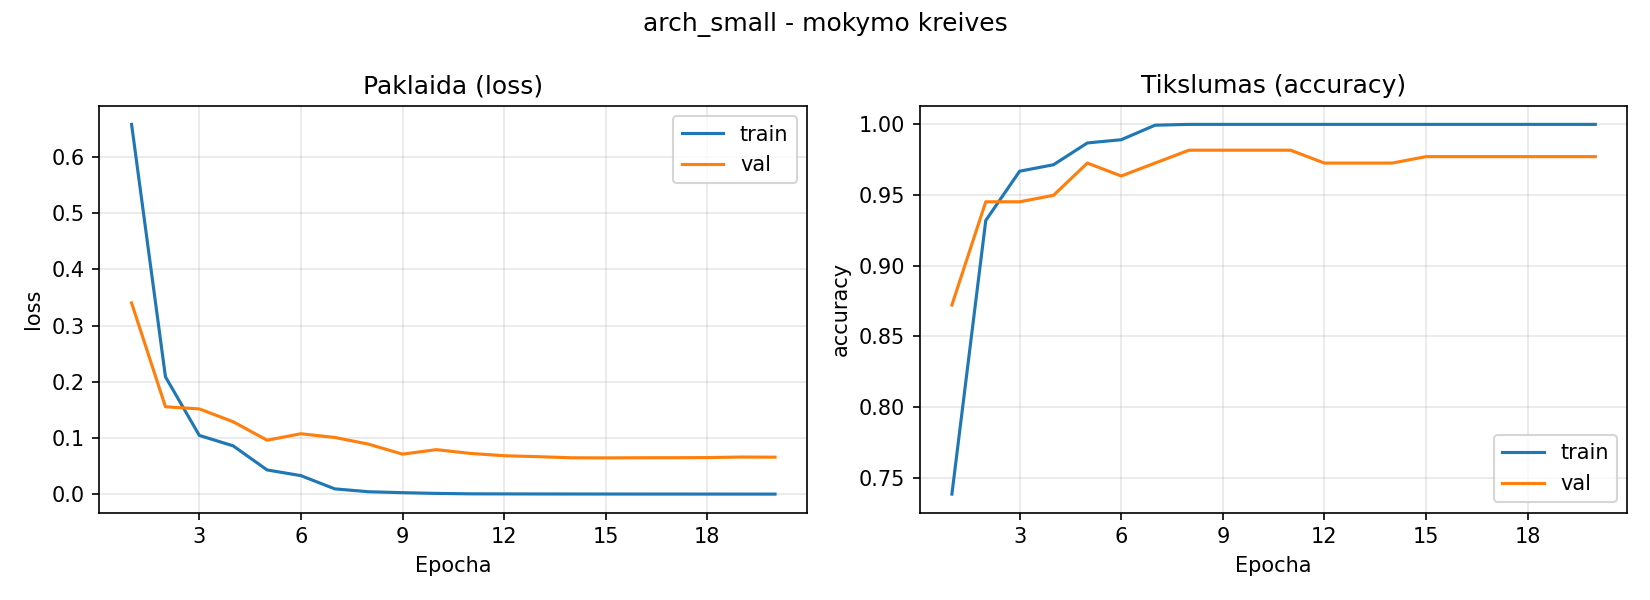
\includegraphics[width=0.85\textwidth]{images/img_arch_small.png}
    \caption{Vaizdai: \texttt{arch\_small} mokymo kreivės}
    \label{fig:img_arch_small}
\end{figure}

\begin{figure}[H]
    \centering
    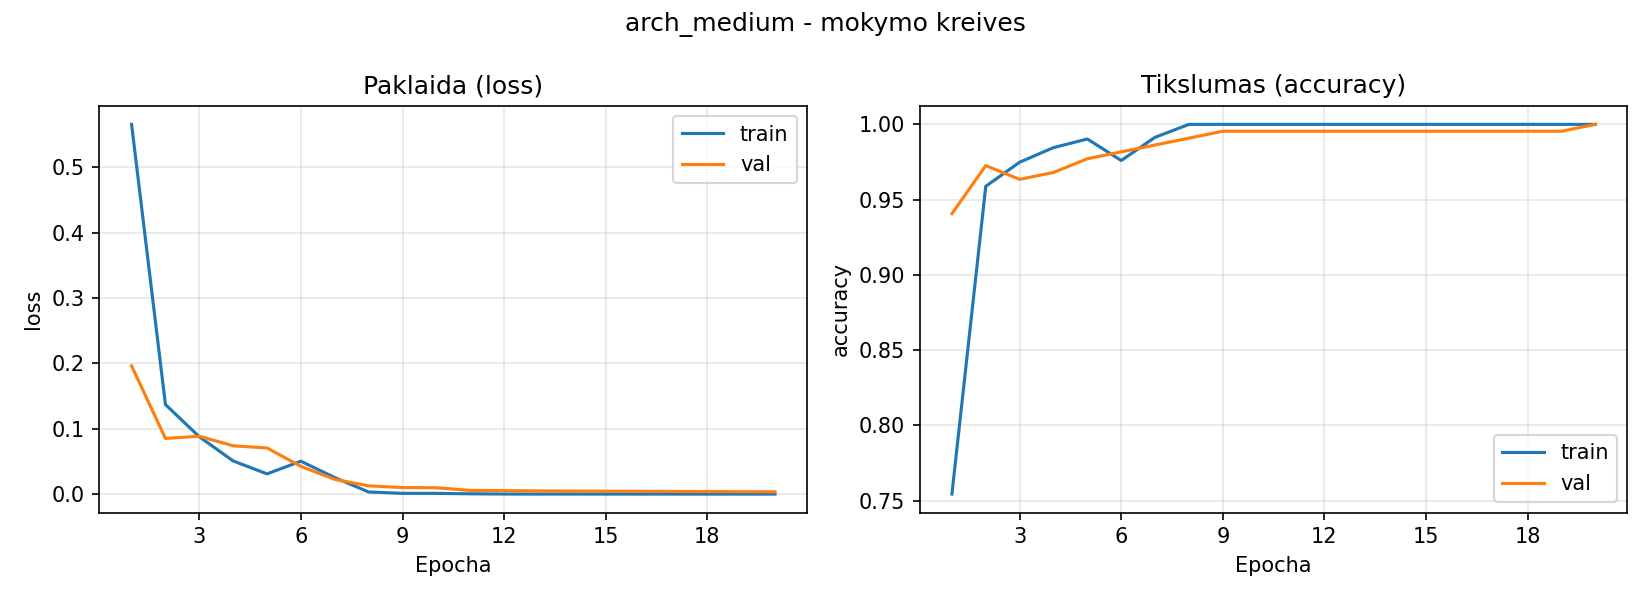
\includegraphics[width=0.85\textwidth]{images/img_arch_medium.png}
    \caption{Vaizdai: \texttt{arch\_medium} mokymo kreivės}
    \label{fig:img_arch_medium}
\end{figure}

\begin{figure}[H]
    \centering
    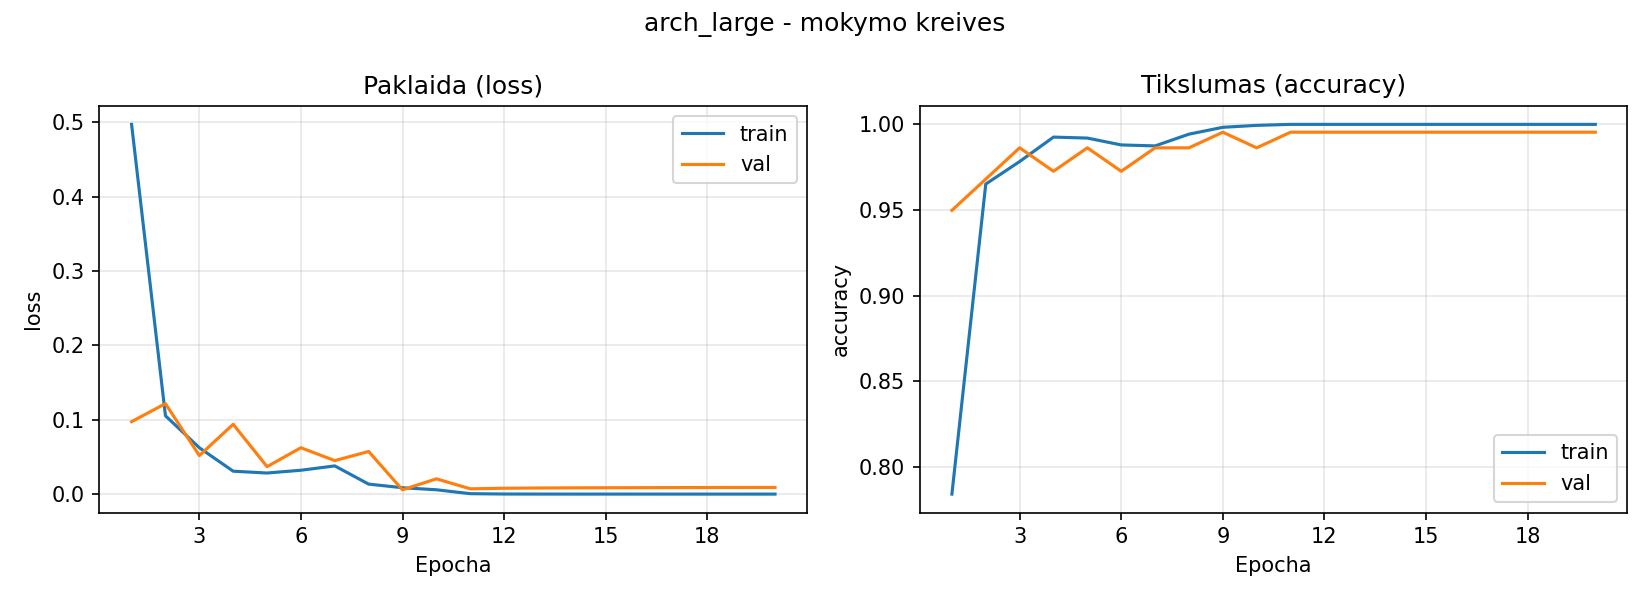
\includegraphics[width=0.85\textwidth]{images/img_arch_large.png}
    \caption{Vaizdai: \texttt{arch\_large} mokymo kreivės}
    \label{fig:img_arch_large}
\end{figure}

Visos trys architektūros pasiekia 100~\% mokymo tikslumą, o validavimo aibėje skiriasi tik nedaug. \texttt{arch\_medium} pasiekia geriausią validavimo tikslumą (\(1{,}0000\)) ir mažiausią validavimo paklaidą. Tolesniems hiperparametrų tyrimams pasirenkama būtent ši architektūra.

\subsubsection{Išmetimo (\textit{dropout}) sluoksnio įtaka}

\begin{table}[H]
    \centering
    \caption{Vaizdai: \textit{dropout} tikimybės įtaka tikslumui ir paklaidai}
    \label{tab:img_dropout}
    \begin{tabular}{|l|c|c|c|c|}
        \hline
        \textbf{Eksperimentas} & \textbf{train\_acc} & \textbf{val\_acc} & \textbf{train\_loss} & \textbf{val\_loss}\\
        \hline
        \texttt{dropout\_p0.0}              & 1{,}0000 & 1{,}0000 & 3$\cdot 10^{-5}$ & 0{,}0036\\
        \hline
        \texttt{dropout\_p0.25}             & 1{,}0000 & 0{,}9726 & 0{,}0005 & 0{,}0898\\
        \hline
        \texttt{dropout\_p0.5}              & 0{,}9817 & 0{,}9543 & 0{,}0505 & 0{,}1902\\
        \hline
        \texttt{dropout\_dense\_only\_0.5}  & 1{,}0000 & 0{,}9863 & 0{,}0006 & 0{,}0567\\
        \hline
    \end{tabular}
\end{table}

\begin{figure}[H]
    \centering
    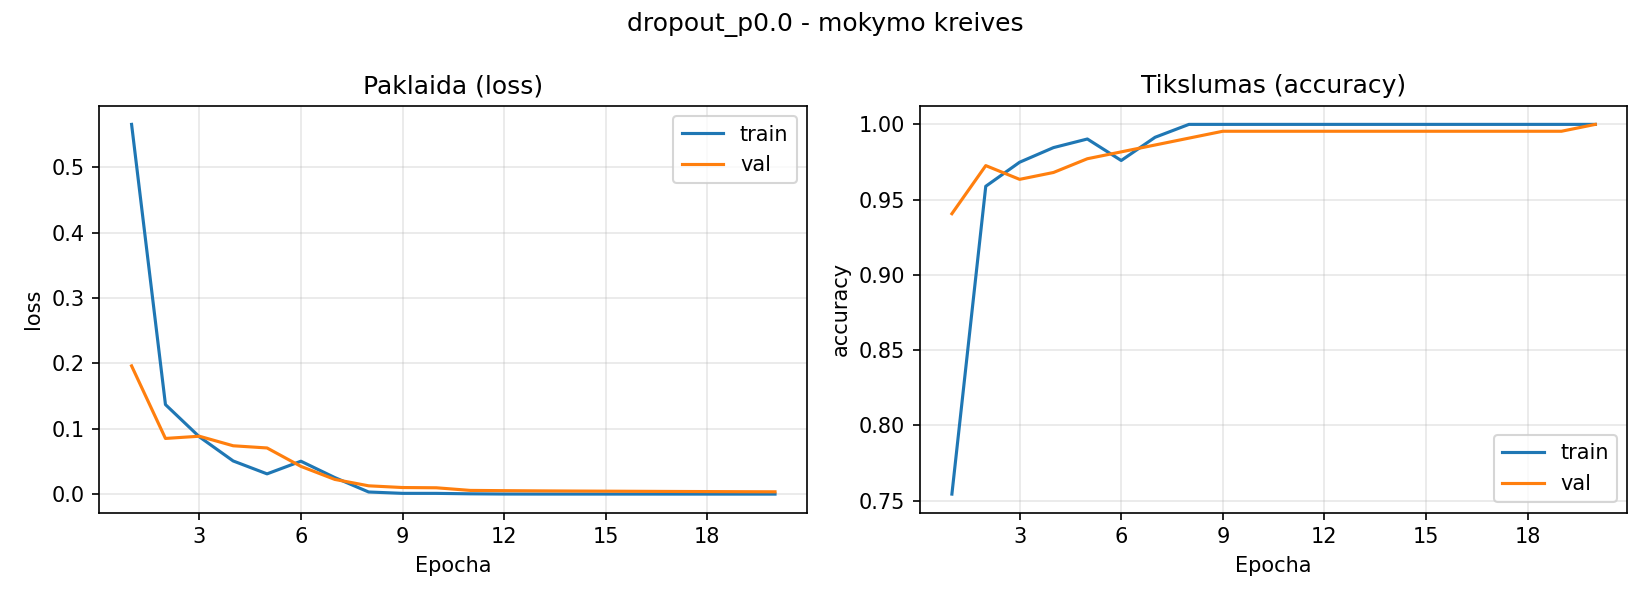
\includegraphics[width=0.85\textwidth]{images/img_dropout_p00.png}
    \caption{Vaizdai: mokymas be \textit{dropout}}
    \label{fig:img_dropout_p00}
\end{figure}

\begin{figure}[H]
    \centering
    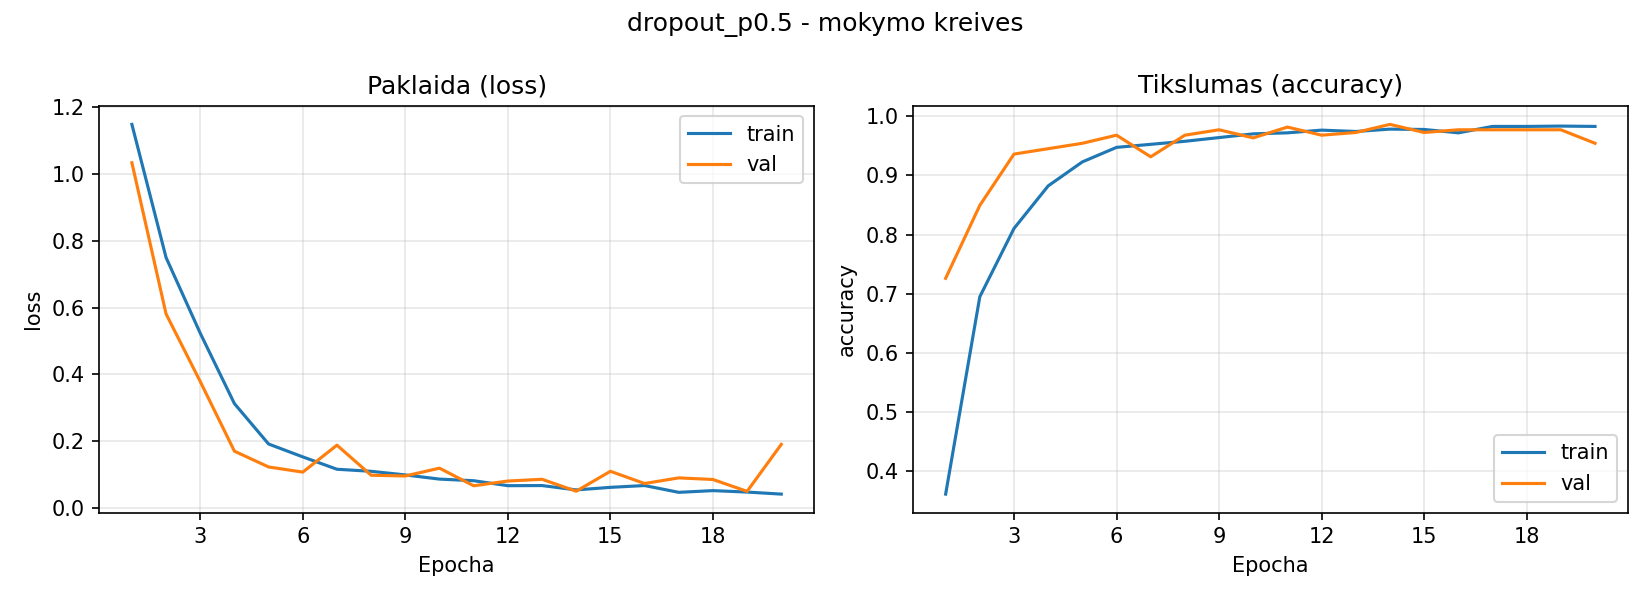
\includegraphics[width=0.85\textwidth]{images/img_dropout_p05.png}
    \caption{Vaizdai: mokymas su stipriu \textit{dropout} (p=0{,}5)}
    \label{fig:img_dropout_p05}
\end{figure}

Mokantis ant paprastų vaizdų rinkinio modelis nepasižymi dideliu persimokymu, todėl agresyvus \textit{dropout} (\(p = 0{,}5\)) reikšmingai sumažina mokymo tikslumą (\(0{,}9817\)) ir blogina validavimo tikslumą (\(0{,}9543\)) bei padidina validavimo paklaidą daugiau nei dvigubai. Vidutinis \(p = 0{,}25\) taip pat šiek tiek blogina validavimo rezultatus. Geriausia šiam uždaviniui \(p = 0\) --- pasiekia tobulą tikslumą; aukšto \textit{dropout} taikymas tik tankiems sluoksniams (\texttt{dense\_only\_0.5}) yra kompromisas, kuris pasižymi mažesniu (98{,}63~\%) validavimo tikslumu.

\subsubsection{Paketų normalizavimo (BN) įtaka}

\begin{table}[H]
    \centering
    \caption{Vaizdai: paketų normalizavimo įtaka}
    \label{tab:img_bn}
    \begin{tabular}{|l|c|c|c|c|}
        \hline
        \textbf{Eksperimentas} & \textbf{train\_acc} & \textbf{val\_acc} & \textbf{train\_loss} & \textbf{val\_loss}\\
        \hline
        \texttt{bn\_off} (be BN) & 1{,}0000 & 1{,}0000 & 3$\cdot 10^{-5}$ & 0{,}0036\\
        \hline
        \texttt{bn\_on}  (su BN) & 1{,}0000 & 1{,}0000 & 0{,}0002 & 0{,}0047\\
        \hline
    \end{tabular}
\end{table}

\begin{figure}[H]
    \centering
    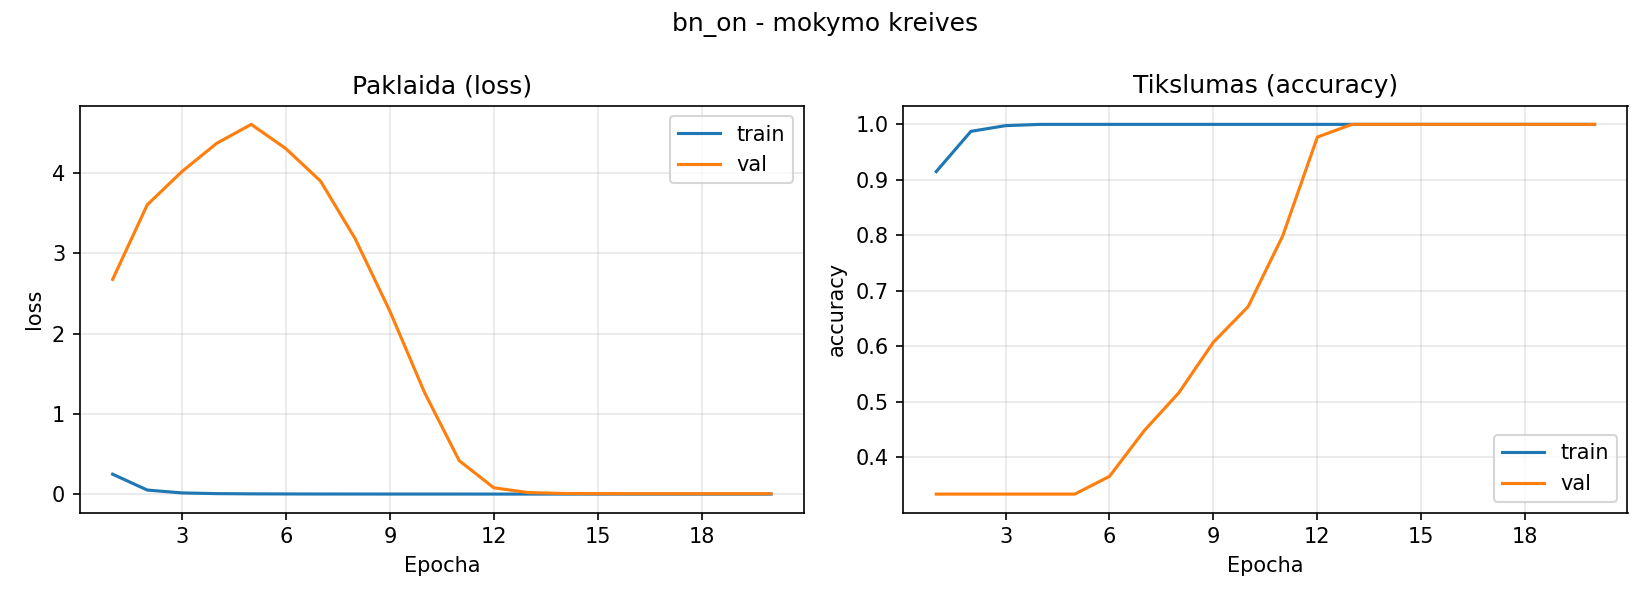
\includegraphics[width=0.85\textwidth]{images/img_bn_on.png}
    \caption{Vaizdai: mokymas su paketų normalizavimu}
    \label{fig:img_bn_on}
\end{figure}

Paketų normalizavimas validavimo aibėje tikslumo praktiškai nekeičia (abu pasiekia \(1{,}0000\)), tačiau šiek tiek padidina mokymo bei validavimo paklaidą. Šiame uždavinyje BN pridėtinės naudos neduoda, modelis ir be jo konverguoja iki tobulo validavimo tikslumo per 20 epochų.

\subsubsection{Aktyvacijos funkcijos įtaka}

\begin{table}[H]
    \centering
    \caption{Vaizdai: aktyvacijos funkcijos palyginimas}
    \label{tab:img_act}
    \begin{tabular}{|l|c|c|c|c|}
        \hline
        \textbf{Aktyvacija} & \textbf{train\_acc} & \textbf{val\_acc} & \textbf{train\_loss} & \textbf{val\_loss}\\
        \hline
        ReLU         & 1{,}0000 & 1{,}0000 & 3$\cdot 10^{-5}$ & 0{,}0036\\
        \hline
        tanh         & 1{,}0000 & 0{,}9954 & 0{,}0012 & 0{,}0133\\
        \hline
        ELU          & 1{,}0000 & 0{,}9909 & 0{,}0002 & 0{,}0446\\
        \hline
        Leaky ReLU   & 1{,}0000 & 0{,}9954 & 3$\cdot 10^{-5}$ & 0{,}0166\\
        \hline
    \end{tabular}
\end{table}

ReLU pasiekia geriausią validavimo tikslumą. Leaky ReLU ir tanh --- nedaug prastesni. ELU šiame uždavinyje šiek tiek atsilieka. Skirtumai tarp aktyvacijų yra triukšmo ribose, todėl gali svyruoti tarp pakartotinių mokymų. \texttt{ChatGPT}.

\subsubsection{Optimizavimo algoritmo įtaka}

\begin{table}[H]
    \centering
    \caption{Vaizdai: optimizatorių palyginimas}
    \label{tab:img_opt}
    \begin{tabular}{|l|c|c|c|c|}
        \hline
        \textbf{Optimizatorius} & \textbf{train\_acc} & \textbf{val\_acc} & \textbf{train\_loss} & \textbf{val\_loss}\\
        \hline
        Adam     & 1{,}0000 & 1{,}0000 & 3$\cdot 10^{-5}$ & 0{,}0036\\
        \hline
        SGD      & 0{,}9903 & 0{,}9909 & 0{,}0287 & 0{,}0345\\
        \hline
        RMSprop  & 1{,}0000 & 0{,}9817 & 1$\cdot 10^{-5}$ & 0{,}0473\\
        \hline
        AdamW    & 1{,}0000 & 1{,}0000 & 3$\cdot 10^{-5}$ & 0{,}0035\\
        \hline
    \end{tabular}
\end{table}

Mokymosi greičio optimizatoriai (Adam, RMSprop, AdamW) duoda labai panašius rezultatus, visi pasiekia tobulą arba beveik tobulą validavimo tikslumą. SGD su tuo pačiu mokymosi greičiu \(\eta = 10^{-3}\) ir \texttt{momentum} = 0{,}9 yra šiek tiek per lėtas konverguoti per 20 epochų, todėl jo mokymo tikslumas atsilieka (\(0{,}9903\)).

\subsection{Laiko eilučių klasifikavimo eksperimentai}

\subsubsection{Architektūrų palyginimas}

\begin{table}[H]
    \centering
    \caption{Laiko eilutės: CNN architektūrų palyginimas}
    \label{tab:ts_arch}
    \begin{tabular}{|l|c|c|c|c|}
        \hline
        \textbf{Modelis} & \textbf{train\_acc} & \textbf{val\_acc} & \textbf{train\_loss} & \textbf{val\_loss}\\
        \hline
        \texttt{arch\_small}  & 1{,}0000 & 0{,}9200 & 0{,}0013 & 0{,}8428\\
        \hline
        \texttt{arch\_medium} & 1{,}0000 & 0{,}9400 & 0{,}0003 & 1{,}2666\\
        \hline
        \texttt{arch\_large}  & 1{,}0000 & 0{,}9133 & 6$\cdot 10^{-5}$ & 0{,}9005\\
        \hline
    \end{tabular}
\end{table}

\begin{figure}[H]
    \centering
    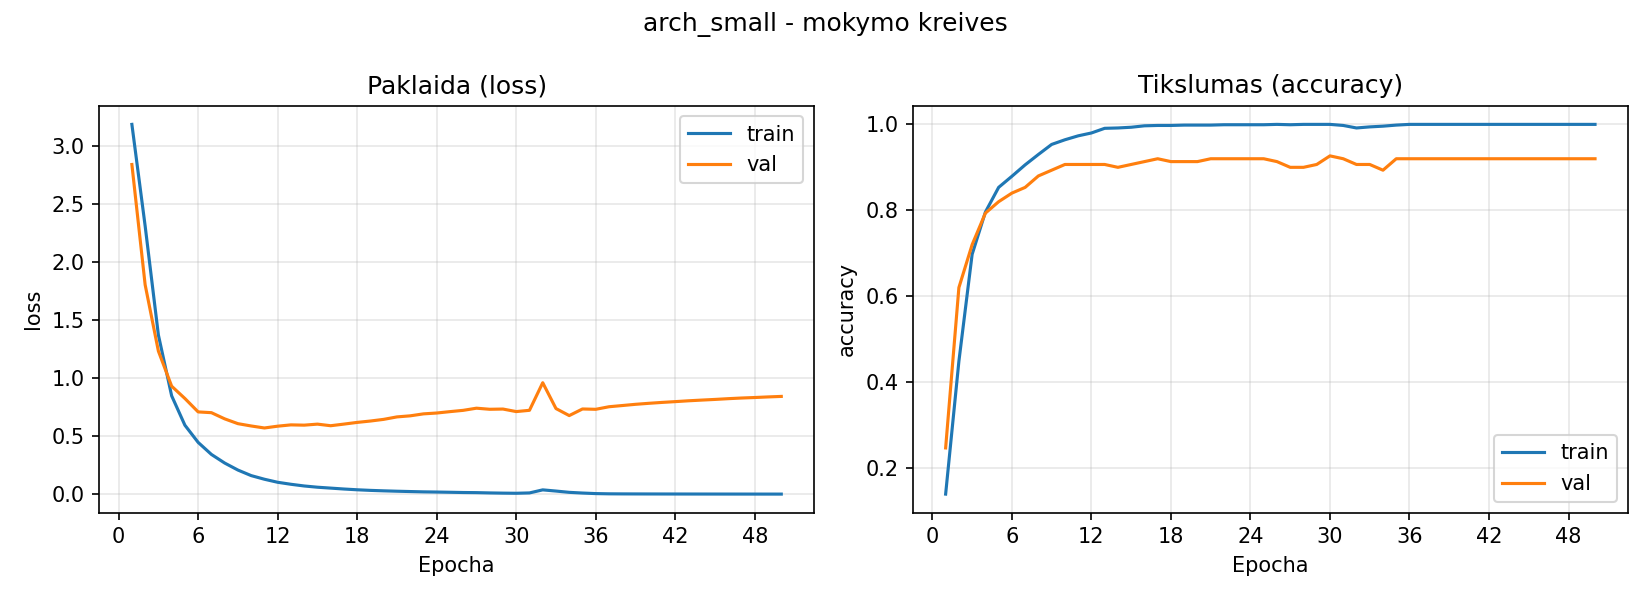
\includegraphics[width=0.85\textwidth]{images/ts_arch_small.png}
    \caption{Laiko eilutės: \texttt{arch\_small} mokymo kreivės}
    \label{fig:ts_arch_small}
\end{figure}

\begin{figure}[H]
    \centering
    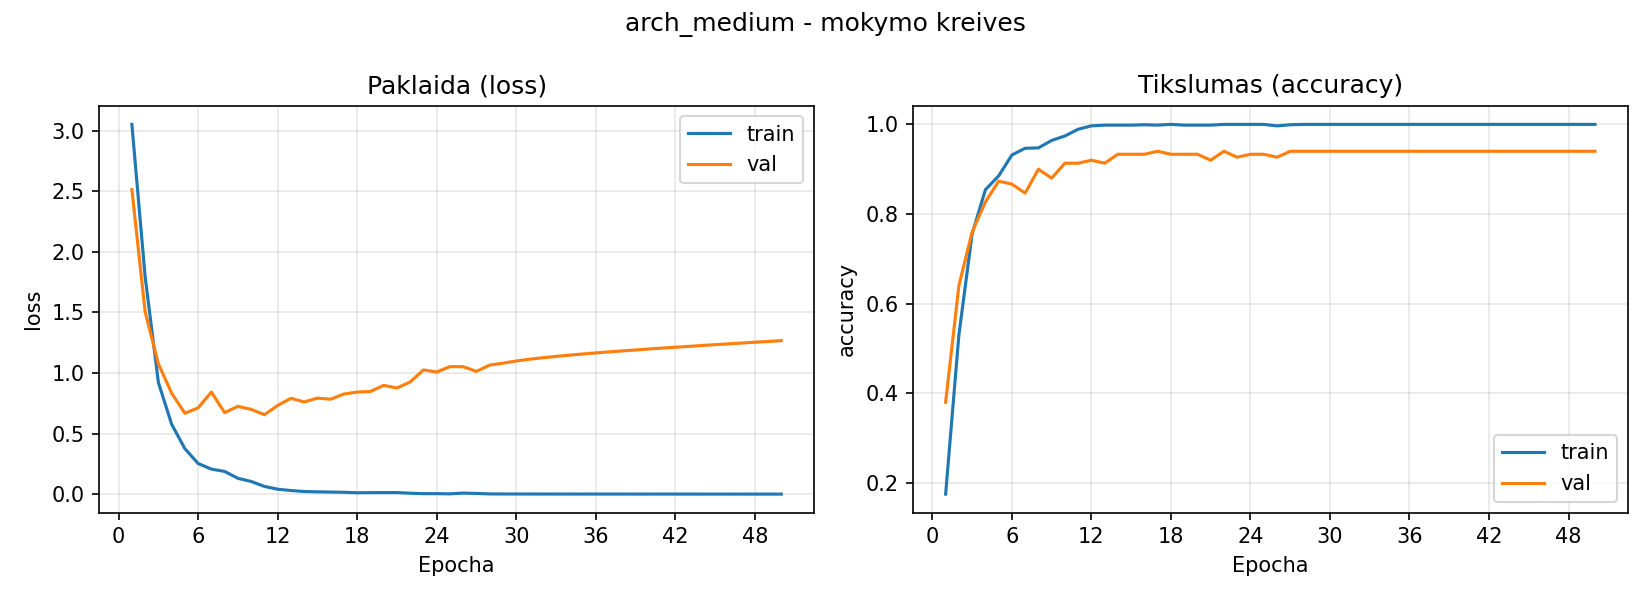
\includegraphics[width=0.85\textwidth]{images/ts_arch_medium.png}
    \caption{Laiko eilutės: \texttt{arch\_medium} mokymo kreivės}
    \label{fig:ts_arch_medium}
\end{figure}

\begin{figure}[H]
    \centering
    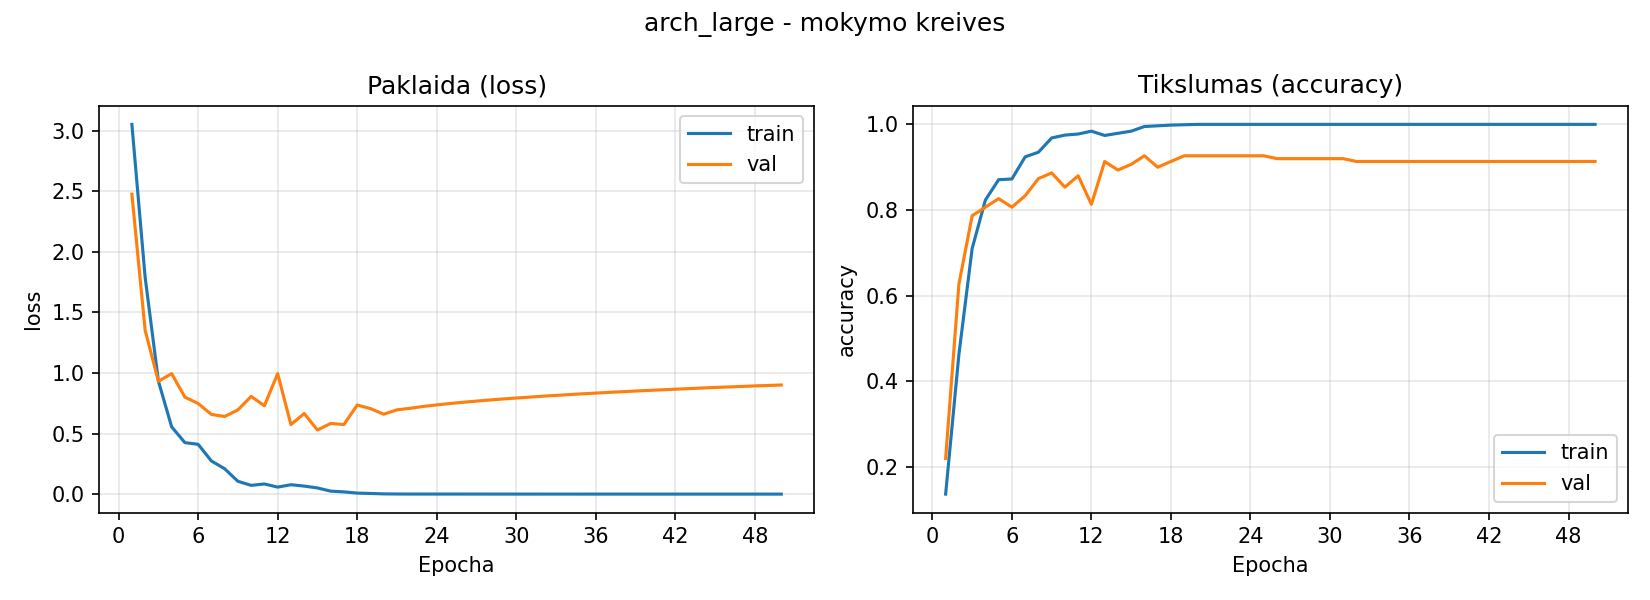
\includegraphics[width=0.85\textwidth]{images/ts_arch_large.png}
    \caption{Laiko eilutės: \texttt{arch\_large} mokymo kreivės}
    \label{fig:ts_arch_large}
\end{figure}

Skirtingai nuo vaizdų, visų trijų architektūrų validavimo tikslumas išlieka apie \(91\)--\(94~\%\). Mokymo aibė įsisavinama tobulai (\(100~\%\)), tačiau didelė validavimo paklaida (iki \(\sim 1{,}27\)) rodo aiškų persimokymą. Validavimo paklaidos kreivė pradeda didėti, nors mokymo paklaida ir toliau krenta. Geriausią validavimo tikslumą pasiekė \texttt{arch\_medium} (\(0{,}9400\)), todėl ji pasirenkama tolesniems hiperparametrų tyrimams.

\subsubsection{Išmetimo (\textit{dropout}) sluoksnio įtaka}

\begin{table}[H]
    \centering
    \caption{Laiko eilutės: \textit{dropout} tikimybės įtaka}
    \label{tab:ts_dropout}
    \begin{tabular}{|l|c|c|c|c|}
        \hline
        \textbf{Eksperimentas} & \textbf{train\_acc} & \textbf{val\_acc} & \textbf{train\_loss} & \textbf{val\_loss}\\
        \hline
        \texttt{dropout\_p0.0}              & 1{,}0000 & 0{,}9400 & 0{,}0003 & 1{,}2666\\
        \hline
        \texttt{dropout\_p0.25}             & 0{,}9992 & 0{,}9400 & 0{,}0051 & 0{,}3771\\
        \hline
        \texttt{dropout\_p0.5}              & 0{,}9742 & 0{,}9267 & 0{,}1588 & 0{,}3479\\
        \hline
        \texttt{dropout\_dense\_only\_0.5}  & 1{,}0000 & 0{,}9333 & 0{,}0025 & 0{,}2485\\
        \hline
    \end{tabular}
\end{table}

\begin{figure}[H]
    \centering
    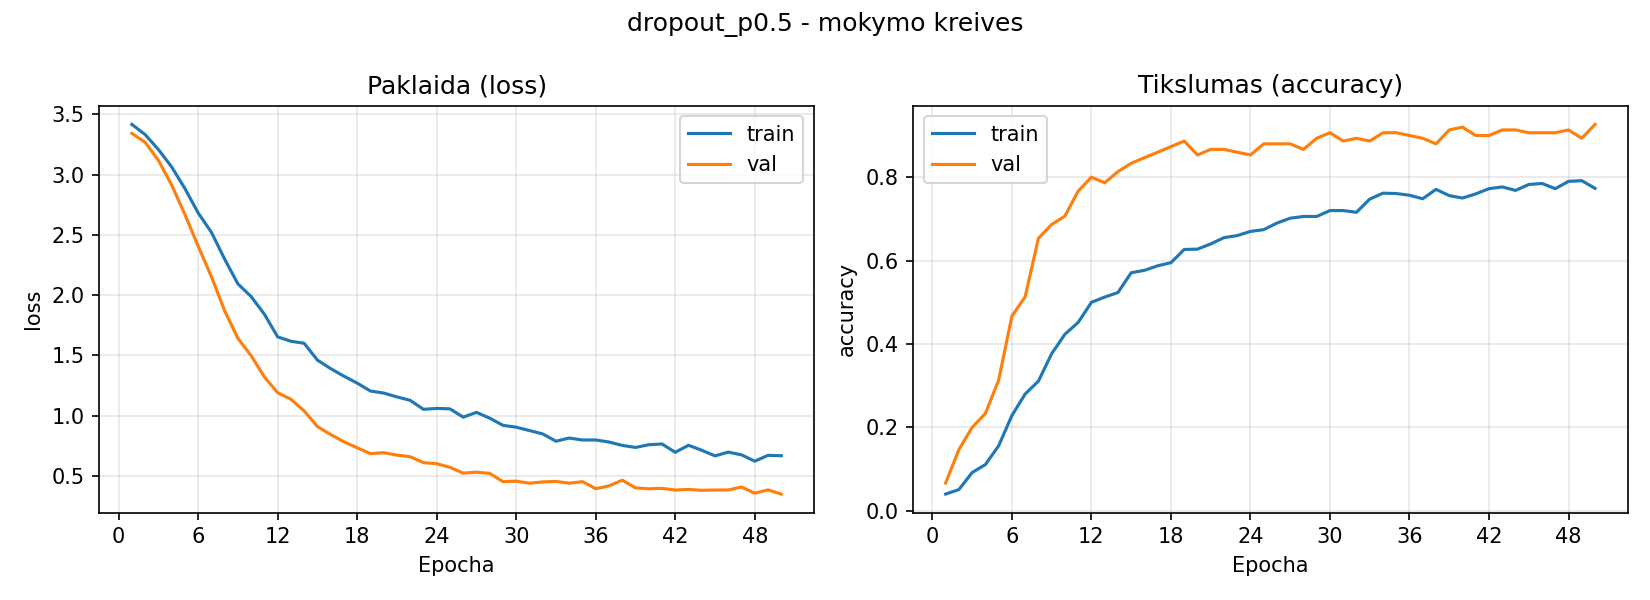
\includegraphics[width=0.85\textwidth]{images/ts_dropout_p05.png}
    \caption{Laiko eilutės: mokymas su \textit{dropout} p=0{,}5}
    \label{fig:ts_dropout_p05}
\end{figure}

Skirtingai nuo vaizdų atvejo, čia \textit{dropout} pridėjimas reikšmingai sumažina validavimo paklaidą (nuo \(1{,}2666\) iki \(\sim 0{,}25\)--\(0{,}38\)), išlaikant panašų validavimo tikslumą (\(\sim 93\)--\(94~\%\)).

\subsubsection{Paketų normalizavimo įtaka}

\begin{table}[H]
    \centering
    \caption{Laiko eilutės: paketų normalizavimo įtaka}
    \label{tab:ts_bn}
    \begin{tabular}{|l|c|c|c|c|}
        \hline
        \textbf{Eksperimentas} & \textbf{train\_acc} & \textbf{val\_acc} & \textbf{train\_loss} & \textbf{val\_loss}\\
        \hline
        \texttt{bn\_off} (be BN) & 1{,}0000 & 0{,}9400 & 0{,}0003 & 1{,}2666\\
        \hline
        \texttt{bn\_on}  (su BN) & 1{,}0000 & 0{,}9400 & 0{,}0013 & 0{,}2433\\
        \hline
    \end{tabular}
\end{table}

\begin{figure}[H]
    \centering
    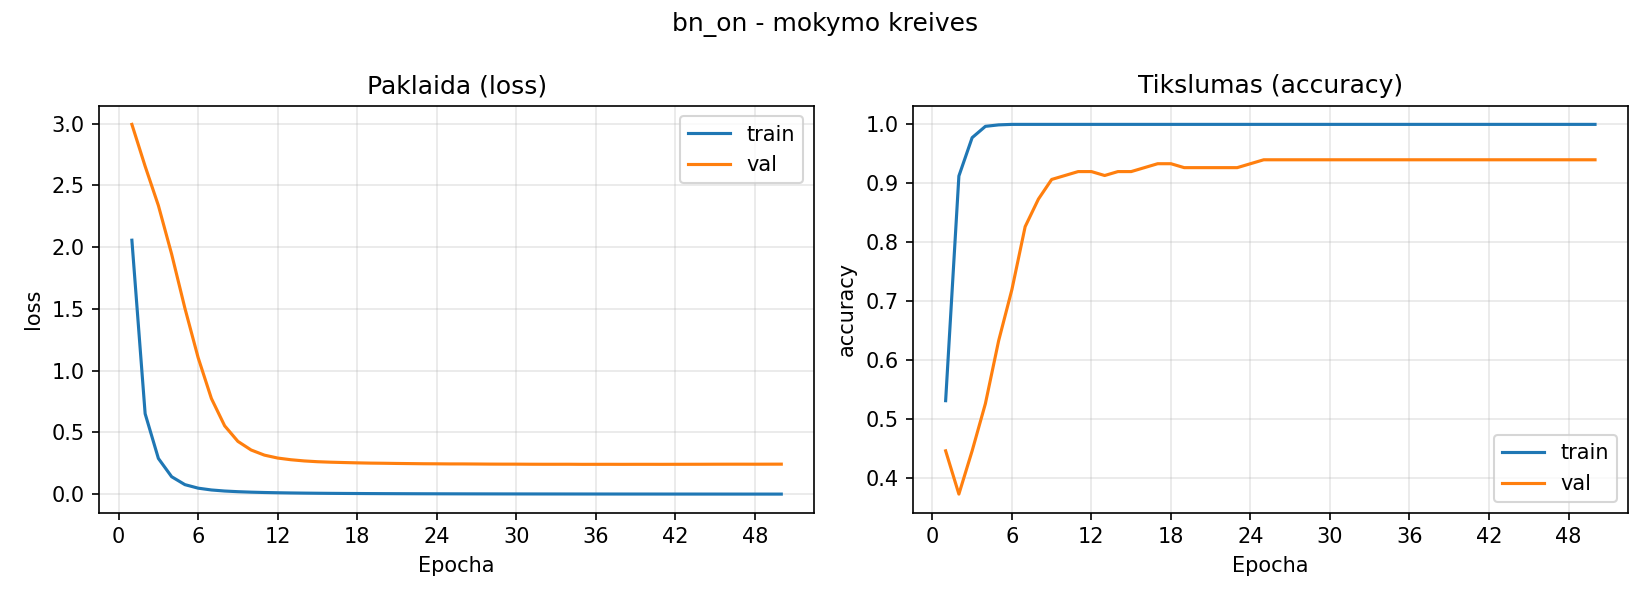
\includegraphics[width=0.85\textwidth]{images/ts_bn_on.png}
    \caption{Laiko eilutės: mokymas su paketų normalizavimu}
    \label{fig:ts_bn_on}
\end{figure}

Šiame uždavinyje BN turi didžiausią poveikį iš visų hiperparametrų: validavimo paklaida sumažėja daugiau nei penkis kartus (nuo \(1{,}2666\) iki \(0{,}2433\)), nors validavimo tikslumas išlieka toks pat (\(0{,}9400\)).

\subsubsection{Aktyvacijos funkcijos įtaka}

\begin{table}[H]
    \centering
    \caption{Laiko eilutės: aktyvacijos funkcijos palyginimas}
    \label{tab:ts_act}
    \begin{tabular}{|l|c|c|c|c|}
        \hline
        \textbf{Aktyvacija} & \textbf{train\_acc} & \textbf{val\_acc} & \textbf{train\_loss} & \textbf{val\_loss}\\
        \hline
        ReLU         & 1{,}0000 & 0{,}9400 & 0{,}0003 & 1{,}2666\\
        \hline
        tanh         & 1{,}0000 & 0{,}9333 & 0{,}0017 & 0{,}2593\\
        \hline
        ELU          & 1{,}0000 & 0{,}9267 & 0{,}0002 & 1{,}1452\\
        \hline
        Leaky ReLU   & 1{,}0000 & 0{,}9200 & 0{,}0003 & 0{,}9553\\
        \hline
    \end{tabular}
\end{table}

tanh pasiekia mažiausią validavimo paklaidą (\(0{,}2593\)), o ReLU -- didžiausią (\(1{,}2666\)); validavimo tikslumas svyruoja nuo \(0{,}9200\) (Leaky ReLU) iki \(0{,}9400\) (ReLU).

\subsubsection{Optimizavimo algoritmo įtaka}

\begin{table}[H]
    \centering
    \caption{Laiko eilutės: optimizatorių palyginimas}
    \label{tab:ts_opt}
    \begin{tabular}{|l|c|c|c|c|}
        \hline
        \textbf{Optimizatorius} & \textbf{train\_acc} & \textbf{val\_acc} & \textbf{train\_loss} & \textbf{val\_loss}\\
        \hline
        Adam     & 1{,}0000 & 0{,}9400 & 0{,}0003 & 1{,}2666\\
        \hline
        SGD      & 0{,}9550 & 0{,}8867 & 0{,}1972 & 0{,}8219\\
        \hline
        RMSprop  & 1{,}0000 & 0{,}9333 & 1$\cdot 10^{-5}$ & 1{,}2656\\
        \hline
        AdamW    & 1{,}0000 & 0{,}9400 & 0{,}0003 & 1{,}2520\\
        \hline
    \end{tabular}
\end{table}

Visi optimizatoriai duoda panašų validavimo tikslumą (\(93\)--\(94~\%\)), o SGD vėl atsilieka tiek mokymo, tiek validavimo aibėse. RMSprop pasiekia mažiausią mokymo paklaidą (\(\approx 10^{-5}\)) ir kartu didžiausią mokymo aibės tikslumą, todėl būtent šis modelis pasirenkamas galutiniam įvertinimui.


\section{Geriausių modelių vertinimas}\label{sec:geriausias}

Geriausiu laikomas tas eksperimentas, kuriame mokymo aibei pasiekiamas didžiausias tikslumas ir mažiausia paklaida. Abiejuose uždaviniuose tokiu pasirodė keičiant optimizatorių į \texttt{RMSprop}. Toliau šie modeliai įvertinami testavimo aibėje.

\subsection{Vaizdų geriausias modelis}

Geriausio vaizdų modelio su \texttt{RMSprop} charakteristikos:
\begin{itemize}
    \item Mokymo tikslumas: \(1{,}0000\), mokymo paklaida: \(\approx 0\);
    \item Validavimo tikslumas: \(1{,}0000\), validavimo paklaida: \(0{,}0473\);
    \item \textbf{Testavimo tikslumas: \(0{,}9817\)}, testavimo paklaida: \(0{,}1420\).
\end{itemize}

\begin{figure}[H]
    \centering
    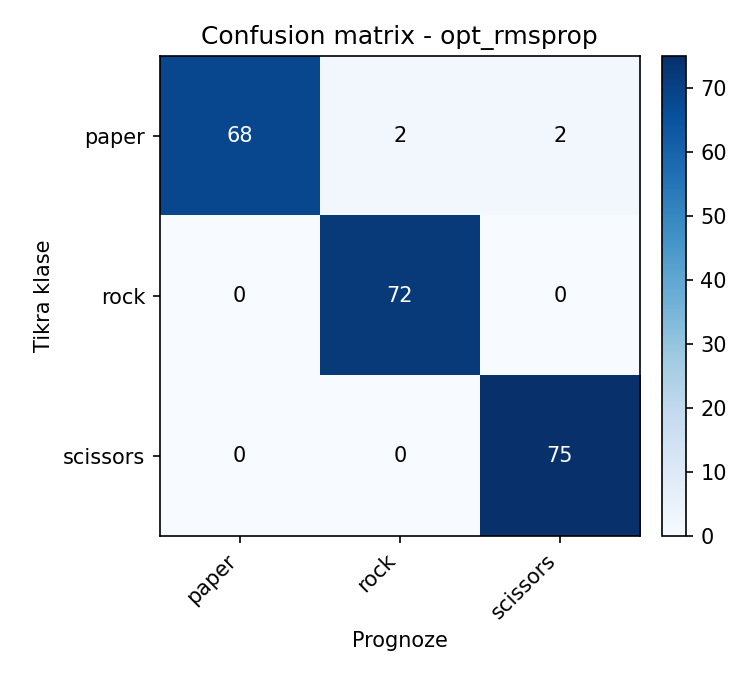
\includegraphics[width=0.6\textwidth]{images/img_confusion.png}
    \caption{Vaizdų geriausio modelio \texttt{confusion matrix} testavimo aibėje}
    \label{fig:img_cm}
\end{figure}

Iš \(219\) testavimo vaizdų teisingai klasifikuoti \(215\). Visos \(4\) klaidos --- klasės \texttt{paper} įrašai, kuriuos modelis suklasifikavo kaip \texttt{rock} (\(2\)) ar \texttt{scissors} (\(2\)). Klasės \texttt{rock} ir \texttt{scissors} testavime atpažintos be klaidų.

\subsubsection{30 testavimo pavyzdžių}

Iš testavimo aibės atrinkta po 10 pavyzdžių iš kiekvienos klasės, iš viso 30 (žr. \ref{fig:img_samples}~pav.). Visi 30 parinktų vaizdų klasifikuoti teisingai (žaliai pažymėtos antraštės). Klaidos pasitaikė tik \texttt{paper} klasėje, kurios atsitiktinai nepateko į šį 30 įrašų poaibį.

\begin{figure}[H]
    \centering
    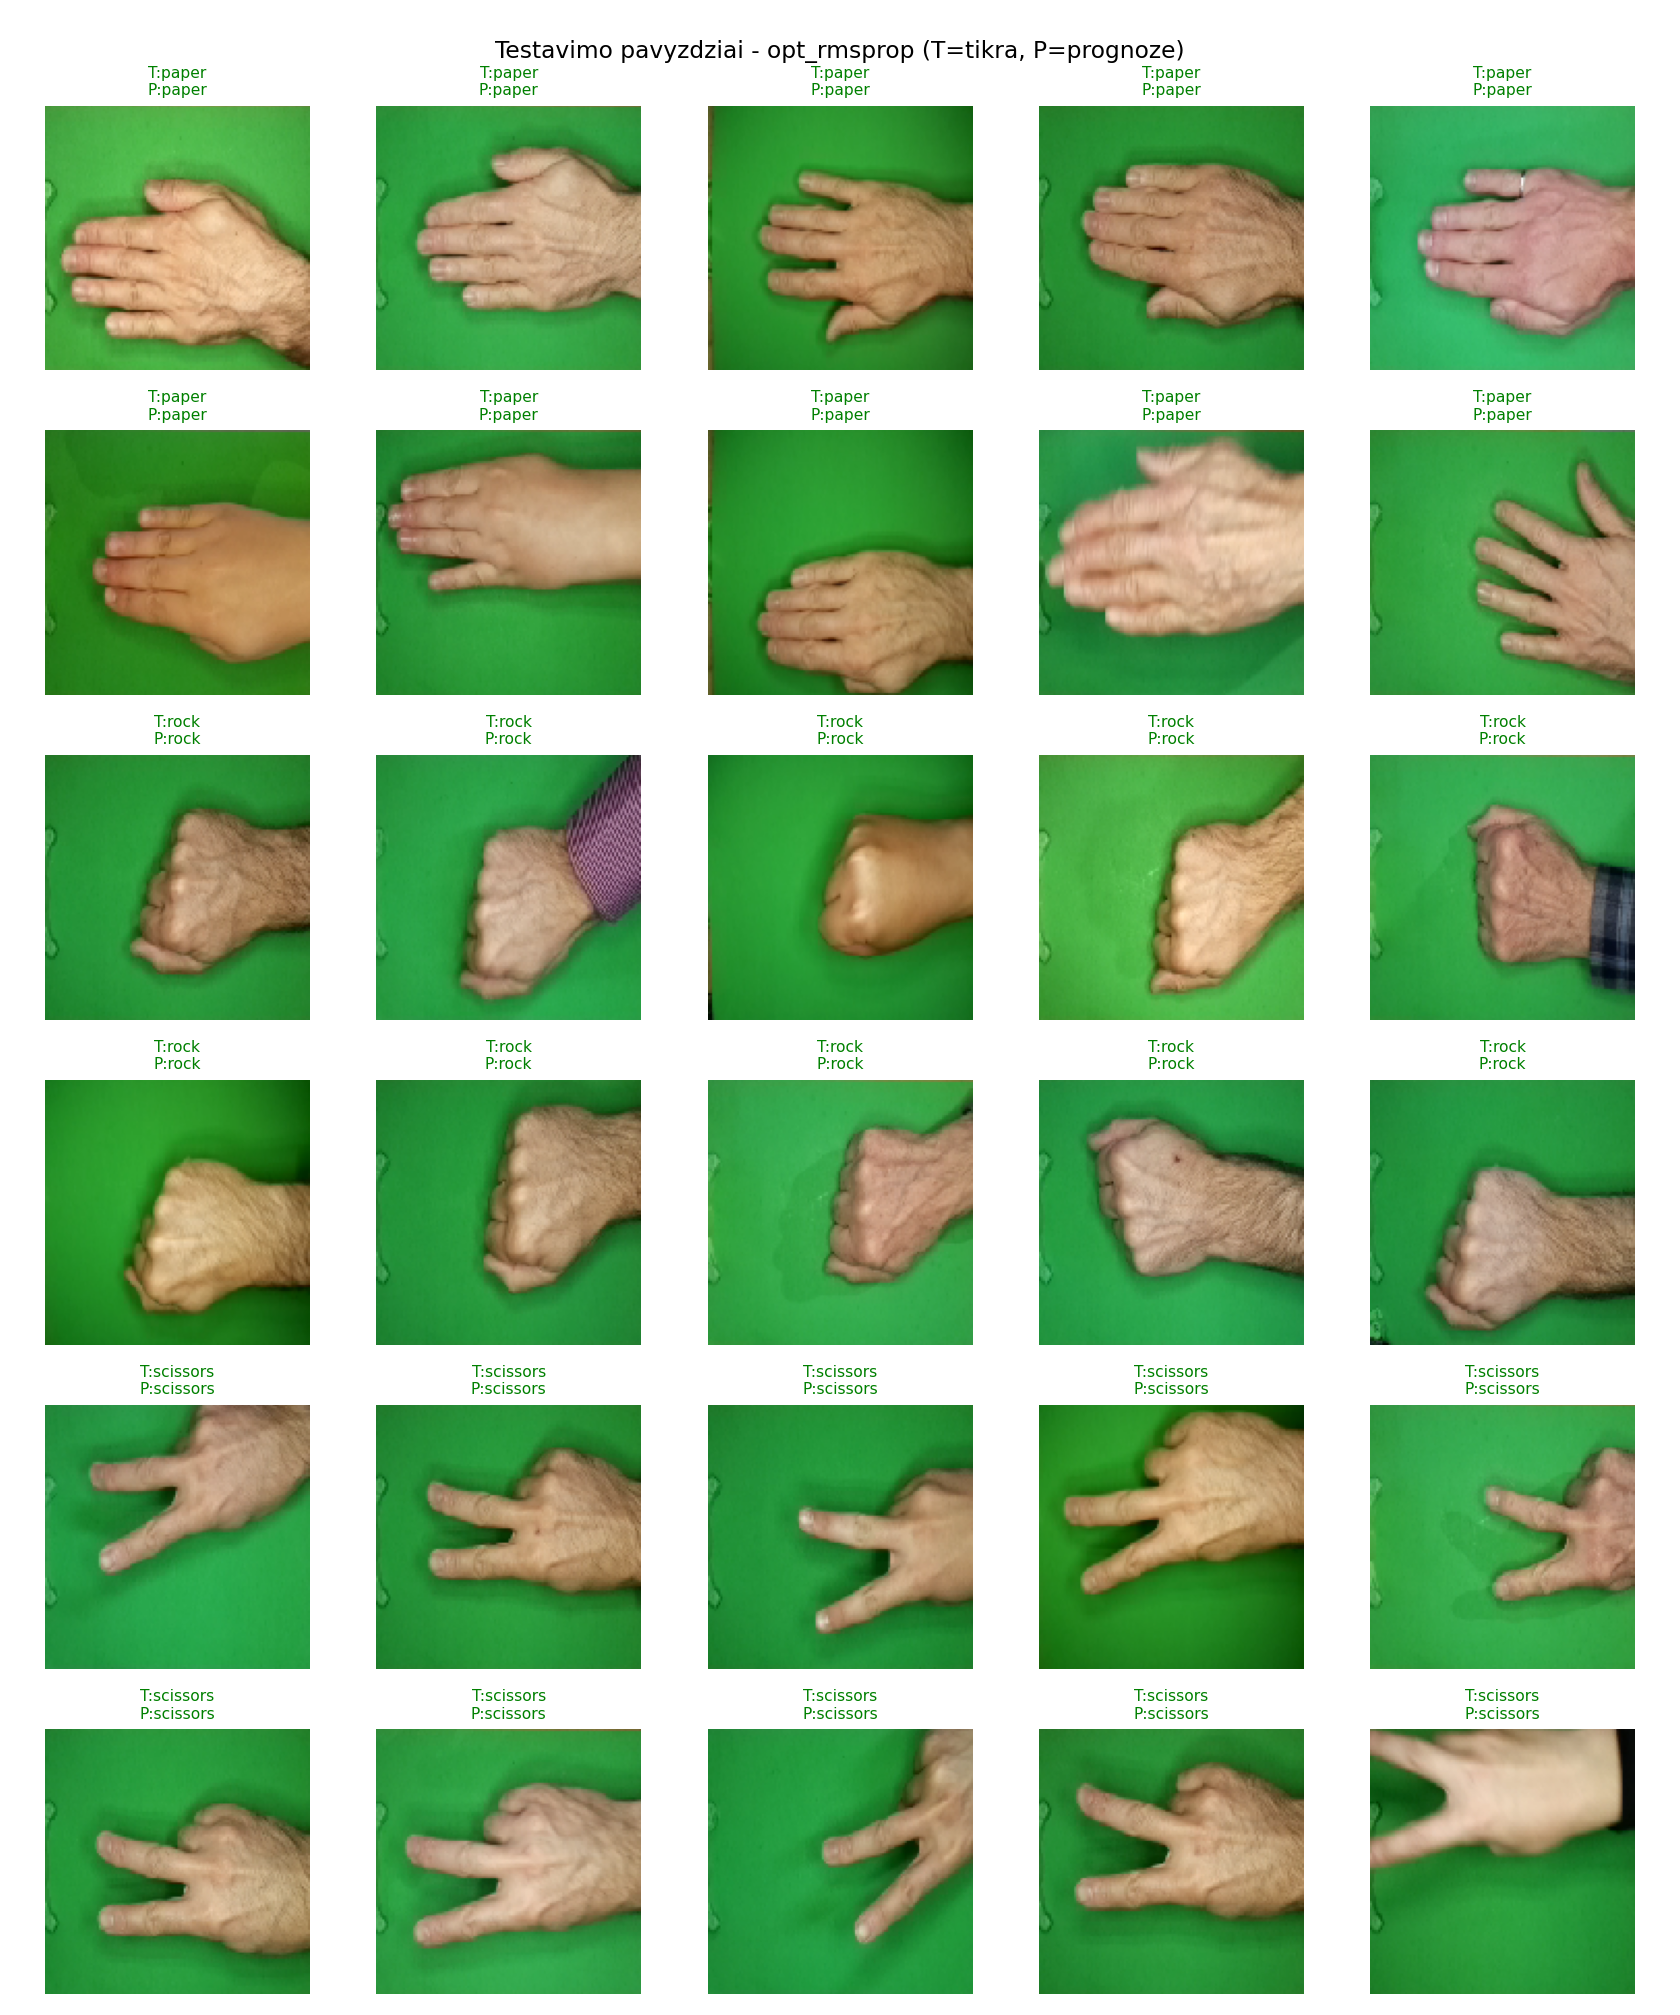
\includegraphics[width=0.95\textwidth]{images/img_samples.png}
    \caption{Vaizdų geriausio modelio prognozės 30 testavimo pavyzdžių. ,,T“ --- tikra klasė, ,,P“ --- prognozė; žalia spalva žymi teisingą klasifikavimą}
    \label{fig:img_samples}
\end{figure}

\subsection{Laiko eilučių geriausias modelis}

Geriausio laiko eilučių modelio su \texttt{RMSprop} charakteristikos:
\begin{itemize}
    \item Mokymo tikslumas: \(1{,}0000\), mokymo paklaida: \(\approx 10^{-5}\);
    \item Validavimo tikslumas: \(0{,}9333\), validavimo paklaida: \(1{,}2656\);
    \item \textbf{Testavimo tikslumas: \(0{,}8800\)}, testavimo paklaida: \(1{,}0788\).
\end{itemize}

\begin{figure}[H]
    \centering
    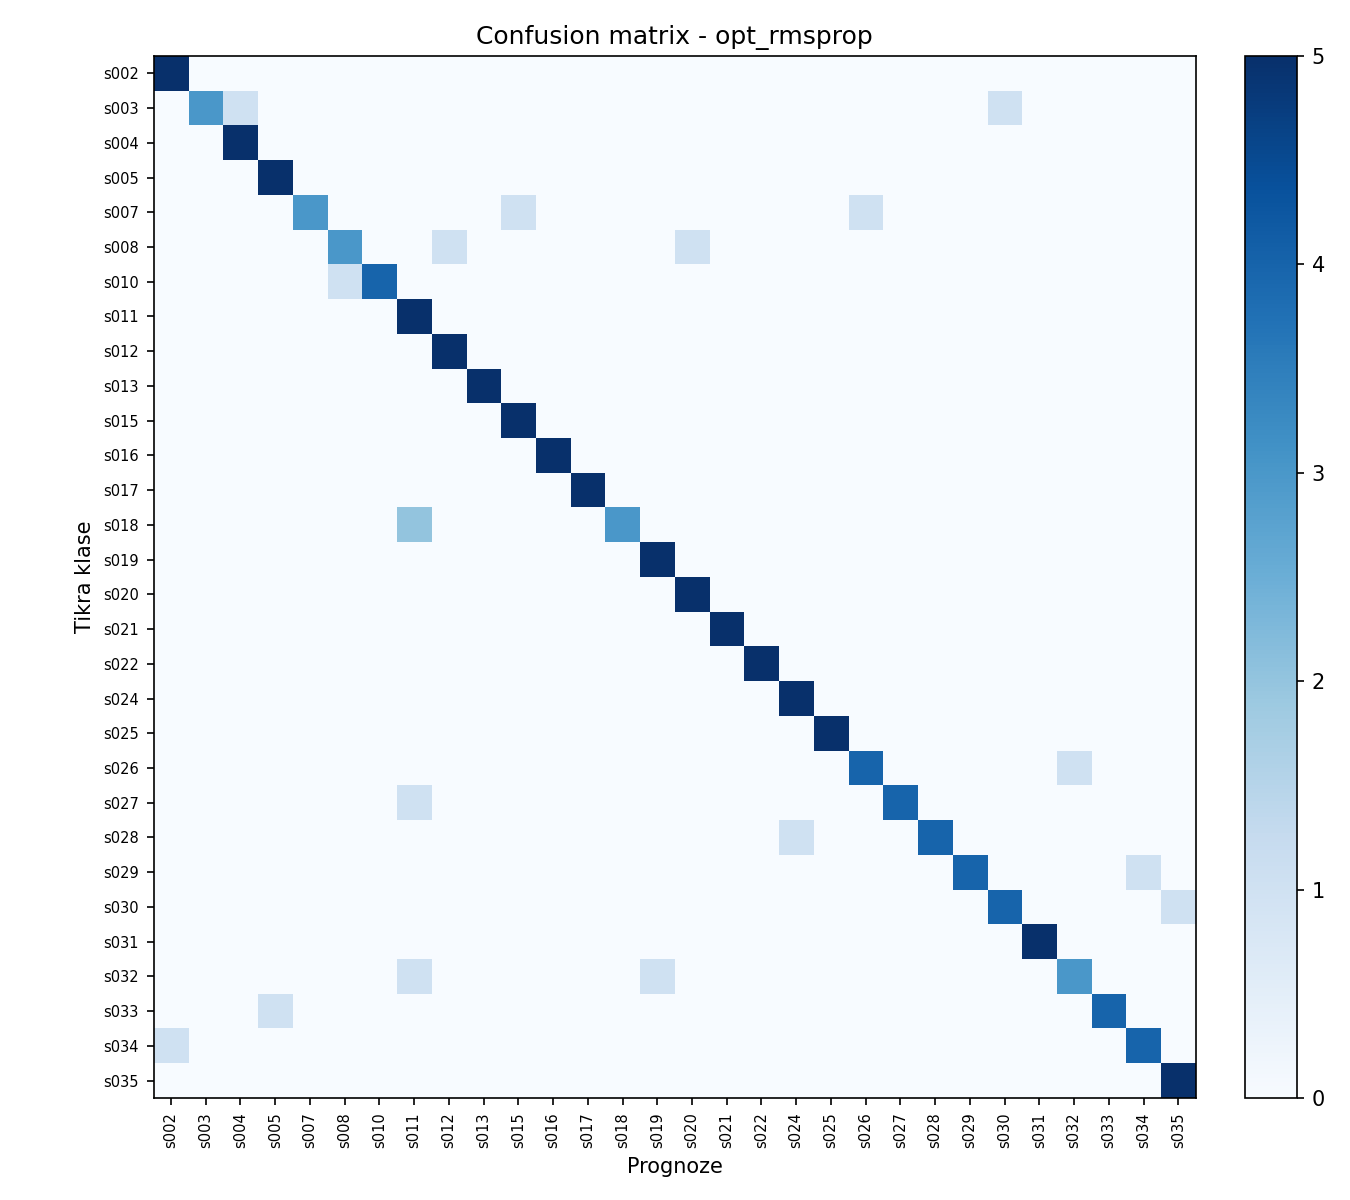
\includegraphics[width=0.95\textwidth]{images/ts_confusion.png}
    \caption{Laiko eilučių geriausio modelio \texttt{confusion matrix}}
    \label{fig:ts_cm}
\end{figure}

\texttt{Confusion matrix} (\(30 \times 30\)) matomos klaidos --- pavienės. Pa vyzdžiui, dalyvis \texttt{s003} kartą suklasifikuotas kaip \texttt{s004}, o \texttt{s007} --- kartą kaip \texttt{s015}. Tai rodo, kad nors atskiros poros dalyvių rašymo tempu yra panašios, sistemiškai blogo klasifikavimo nėra.

\subsubsection{30 testavimo pavyzdžių}

Iš testavimo aibės parinktas vienas įrašas iš kiekvienos iš \(30\) klasių. Lentelėje~\ref{tab:ts_samples} parodytos tikros ir prognozuotos klasės; iš \(30\) pavyzdžių \(28\) klasifikuoti teisingai, \(2\) --- klaidingai (\texttt{s003} -- \texttt{s004}, \texttt{s007} -- \texttt{s015}). Tai duoda \(\sim 93~\%\) tikslumą šio mažo poaibio.

\begin{table}[H]
    \centering
    \caption{Laiko eilutės: geriausio modelio prognozės 30-čiai testavimo pavyzdžių (po 1 iš kiekvienos klasės)}
    \label{tab:ts_samples}
    \begin{tabular}{|c|c|c|c|}
        \hline
        \textbf{Nr.} & \textbf{Tikras dalyvis} & \textbf{Prognozė} & \textbf{Teisinga?}\\
        \hline
        1  & s002 & s002 & taip \\ \hline
        2  & s003 & s004 & ne   \\ \hline
        3  & s004 & s004 & taip \\ \hline
        4  & s005 & s005 & taip \\ \hline
        5  & s007 & s015 & ne   \\ \hline
        6  & s008 & s008 & taip \\ \hline
        7  & s010 & s010 & taip \\ \hline
        8  & s011 & s011 & taip \\ \hline
        9  & s012 & s012 & taip \\ \hline
        10 & s013 & s013 & taip \\ \hline
        11 & s015 & s015 & taip \\ \hline
        12 & s016 & s016 & taip \\ \hline
        13 & s017 & s017 & taip \\ \hline
        14 & s018 & s018 & taip \\ \hline
        15 & s019 & s019 & taip \\ \hline
        16 & s020 & s020 & taip \\ \hline
        17 & s021 & s021 & taip \\ \hline
        18 & s022 & s022 & taip \\ \hline
        19 & s024 & s024 & taip \\ \hline
        20 & s025 & s025 & taip \\ \hline
        21 & s026 & s026 & taip \\ \hline
        22 & s027 & s027 & taip \\ \hline
        23 & s028 & s028 & taip \\ \hline
        24 & s029 & s029 & taip \\ \hline
        25 & s030 & s030 & taip \\ \hline
        26 & s031 & s031 & taip \\ \hline
        27 & s032 & s032 & taip \\ \hline
        28 & s033 & s033 & taip \\ \hline
        29 & s034 & s034 & taip \\ \hline
        30 & s035 & s035 & taip \\ \hline
    \end{tabular}
\end{table}


\sectionnonum{Išvados}

Konvoliuciniai neuroniniai tinklai sėkmingai pritaikyti abiem skirtingo tipo uždaviniams: vaizdų klasifikavimui (3 klasės) ir biometrinių laiko eilučių klasifikavimui (30 klasių). Iš trijų lygintų architektūrų \texttt{arch\_medium} (3 konvoliuciniai blokai, vienas tankus sluoksnis) pasižymėjo geriausiai abiems uždaviniams, gilesnis tinklas papildomos naudos neduoda, o paprastesnis tampa nestabilus. Vaizdų uždavinyje stiprus \textit{dropout} (\(p = 0{,}5\)) blogina rezultatus, nes modelis nepatiria didelio persimokymo, o laiko eilučių uždavinyje \textit{dropout} (\(p \in \{0{,}25;\ 0{,}5\}\)) reikšmingai sumažina paklaidą ir padidina testavimo tikslumą iki \(\sim 91~\%\). Paketų normalizavimas labiausiai naudingas laiko eilutėms (testavimo tikslumas padidėjo nuo \(86~\%\) iki \(93{,}33~\%\), o paklaida sumažėjo nuo \(0{,}886\) iki \(0{,}210\)), vaizdams paklaidą sumažino, bet tikslumo praktiškai nepakeitė. Aktyvacijos funkcijos turi mažesnę įtaką: ReLU, Leaky ReLU ir tanh duoda panašų vaizdų tikslumą, tuo tarpu, laiko eilutėms tanh sumažino paklaidą. Optimizatoriai (Adam, RMSprop, AdamW) duoda panašius rezultatus, o SGD su \(\eta = 10^{-3}\). Didžiausias mokymo tikslumas (\(1{,}0000\)) ir mažiausia mokymo paklaida (\(\approx 0\) vaizdams, \(\approx 10^{-5}\) laiko eilutėms) gauti su \texttt{RMSprop} konfigūracija abiem uždaviniams, todėl būtent ji parinkta galutiniam vertinimui testavimo aibėje. Geriausio vaizdų modelio testavimo tikslumas --- \(98{,}17~\%\) (paklaida \(0{,}142\)), visi keturi klaidingi atvejai yra klasės \texttt{paper} prognozavimas kaip \texttt{rock}/\texttt{scissors}, \texttt{rock} ir \texttt{scissors} atpažintos be klaidų. Geriausio laiko eilučių modelio testavimo tikslumas --- \(88{,}00~\%\) (paklaida \(1{,}079\)), o \texttt{confusion matrix} rodo jog klaidos pavienės ir pasiskirsčiusios. Iš 30 atrinktų testavimo pavyzdžių vaizdams visi (\(30/30\)) klasifikuoti teisingai, o laiko eilutėms --- \(28/30\). Bendras darbo rezultatas patvirtina, kad parametrizuotas CNN karkasas su nedidele paketų normalizavimo ir \textit{dropout} panaudojimu yra paprastas ir efektyvus sprendimas tiek vaizdo, tiek laiko eilučių klasifikacijos uždaviniams.


\printbibliography[title = {Literatūra ir šaltiniai}]


\appendix
\renewcommand{\thesection}{\arabic{section} priedas.}

\section{\phantom{Priedas} Vaizdų klasifikavimo programa (\texttt{main.py})}\label{app:main}

Žemiau pateikiamas pilnas vaizdų klasifikavimo programos kodas.

\begin{verbatim}
import csv
import os
import random
import sys
from copy import deepcopy
from pathlib import Path

os.environ.setdefault("TF_CPP_MIN_LOG_LEVEL", "2")
os.environ.setdefault("TF_ENABLE_ONEDNN_OPTS", "0")

import matplotlib

matplotlib.use("Agg")
import matplotlib.pyplot as plt
from matplotlib.ticker import MaxNLocator
import numpy as np
import tensorflow as tf
from sklearn.metrics import confusion_matrix
from sklearn.model_selection import train_test_split
from tensorflow.keras import layers, models, optimizers

# Konfiguracija
SEED = 42
random.seed(SEED)
np.random.seed(SEED)
tf.random.set_seed(SEED)

CW_DIR = Path(__file__).resolve().parent
DATA_DIR = CW_DIR / "rockpaperscissors"
RESULTS_DIR = CW_DIR / "rezultatai" / "images"
RESULTS_DIR.mkdir(parents=True, exist_ok=True)

CLASS_NAMES = ["paper", "rock", "scissors"] 
IMG_SIZE = (128, 128)  # H x W - sumazinta is originalo (300x200), kad tilptu i atminti
NUM_CLASSES = len(CLASS_NAMES)
SUMMARY_CSV = RESULTS_DIR / "summary.csv"


# Duomenu paruosimas
def load_images() -> tuple[np.ndarray, np.ndarray, list[str]]:
    #Iskraunam visus PNG i atminti, normalizuojam i [0,1].
    X, y, paths = [], [], []
    for label_idx, cname in enumerate(CLASS_NAMES):
        cdir = DATA_DIR / cname
        files = sorted(cdir.glob("*.png"))
        for fp in files:
            img = tf.keras.utils.load_img(str(fp), target_size=IMG_SIZE)
            arr = tf.keras.utils.img_to_array(img) / 255.0  # float32 [0,1]
            # nuotraukų pixelių masyvai
            X.append(arr)
            # klasių masyvas
            y.append(label_idx)
            paths.append(str(fp))
    # Chat gpt. 3D masyvų masyvas N x (H x W x 3) -> 4D masyvą (N x H x W x 3) (tensorius) 
    X = np.asarray(X, dtype=np.float32)
    y = np.asarray(y, dtype=np.int64)
    return X, y, paths


def make_splits(X: np.ndarray, y: np.ndarray, paths: list[str]):
    #80/10/10 paskirstymas.
    paths = np.asarray(paths)
    # 80% mokymui / 20% like įrašai
    X_tr, X_rest, y_tr, y_rest, p_tr, p_rest = train_test_split(
        X, y, paths, test_size=0.20, stratify=y, random_state=SEED
    )
    # is likusio 20% padalinam per puse -> 10% validacijos / 10% testavimo
    X_va, X_te, y_va, y_te, p_va, p_te = train_test_split(
        X_rest, y_rest, p_rest, test_size=0.50, stratify=y_rest, random_state=SEED
    )
    return (X_tr, y_tr, p_tr), (X_va, y_va, p_va), (X_te, y_te, p_te)

def make_activation_layer(name: str):
    # Pagalbine funkcija del leakyReLU parametro negative_slope
    name = name.lower()
    if name == "leaky_relu":
        return layers.LeakyReLU(negative_slope=0.1)
    return layers.Activation(name)


def _make_optimizer(name: str, lr: float):
    # Pagalbine funkcija del skirtingu parametru
    name = name.lower()
    if name == "adam":
        return optimizers.Adam(learning_rate=lr)
    if name == "sgd":
        return optimizers.SGD(learning_rate=lr, momentum=0.9)
    if name == "rmsprop":
        return optimizers.RMSprop(learning_rate=lr)
    if name == "adamw":
        return optimizers.AdamW(learning_rate=lr)
    raise ValueError(f"Nezinomas optimizatorius: {name}")


def build_model(cfg: dict, input_shape: tuple, num_classes: int) -> tf.keras.Model:
    """Sukuriamas 'keras' modelis pagal cfg

    cfg pavyzdys:
      {
        "blocks": [{"filters":32,"kernel":3,"pool":2,"dropout":0.0,"batch_norm":False,"activation":"relu"}, ...],
        "dense": [128],
        "dense_dropout": 0.0,
        "dense_batch_norm": False,
        "dense_activation": "relu",
        "optimizer": "adam", "learning_rate": 1e-3,
        "loss": "sparse_categorical_crossentropy",
      }


    Input(H, W, 3)
    → [conv2d → (BN?) → activation → (MaxPool?) → (Dropout?)] × len(blocks)
    → Flatten
    → [Dense(units) → (BN?) → activation → (Dropout?)] × len(dense)
    → Dense(num_classes, softmax)
    → compile(loss, optimizer, metrics=accuracy)
    """
    model = models.Sequential(name=cfg["name"].replace(".", "_"))
    model.add(layers.Input(shape=input_shape))

    for i, blk in enumerate(cfg["blocks"]):
        # Conv -> (BN) -> aktyvacija -> Pooling -> (Dropout)
        # use_bias=False kai BN, nes BN turi savo bias.
        use_bias = not blk.get("batch_norm", False)
        model.add(
            layers.Conv2D(
                filters=blk["filters"],
                kernel_size=blk["kernel"],
                padding="same",
                use_bias=use_bias,
                name=f"conv2d_{i}",
            )
        )
        if blk.get("batch_norm", False):
            model.add(layers.BatchNormalization(name=f"bn_{i}"))
        model.add(make_activation_layer(blk["activation"]))
        if blk.get("pool", 0):
            model.add(layers.MaxPooling2D(pool_size=blk["pool"], name=f"pool_{i}"))
        if blk.get("dropout", 0.0) > 0.0:
            model.add(layers.Dropout(blk["dropout"], name=f"drop_{i}"))

    #ChatGpt
    model.add(layers.Flatten())

    for j, units in enumerate(cfg.get("dense", [])):
        model.add(layers.Dense(units, use_bias=not cfg.get("dense_batch_norm", False),
                               name=f"dense_{j}"))
        if cfg.get("dense_batch_norm", False):
            model.add(layers.BatchNormalization(name=f"dense_bn_{j}"))
        model.add(make_activation_layer(cfg.get("dense_activation", "relu")))
        if cfg.get("dense_dropout", 0.0) > 0.0:
            model.add(layers.Dropout(cfg["dense_dropout"], name=f"dense_drop_{j}"))

    model.add(layers.Dense(num_classes, activation="softmax", name="output"))

    model.compile(
        optimizer=_make_optimizer(cfg.get("optimizer", "adam"),
                                  cfg.get("learning_rate", 1e-3)),
        loss=cfg.get("loss", "sparse_categorical_crossentropy"),
        metrics=["accuracy"],
    )
    return model


def plot_history(history, title: str, save_path: Path):
    h = history.history
    epochs = range(1, len(h["loss"]) + 1)
    fig, axes = plt.subplots(1, 2, figsize=(11, 4))

    axes[0].plot(epochs, h["loss"], label="train")
    axes[0].plot(epochs, h["val_loss"], label="val")
    axes[0].set_title("Paklaida (loss)")
    axes[0].set_xlabel("Epocha")
    axes[0].set_ylabel("loss")
    axes[0].legend()
    axes[0].grid(alpha=0.3)
    axes[0].xaxis.set_major_locator(MaxNLocator(integer=True))

    axes[1].plot(epochs, h["accuracy"], label="train")
    axes[1].plot(epochs, h["val_accuracy"], label="val")
    axes[1].set_title("Tikslumas (accuracy)")
    axes[1].set_xlabel("Epocha")
    axes[1].set_ylabel("accuracy")
    axes[1].legend()
    axes[1].grid(alpha=0.3)
    axes[1].xaxis.set_major_locator(MaxNLocator(integer=True))

    fig.suptitle(title)
    fig.tight_layout()
    fig.savefig(save_path, dpi=150)
    plt.close(fig)


def append_summary(row: dict):
    new_file = not SUMMARY_CSV.exists()
    with SUMMARY_CSV.open("a", newline="") as f:
        w = csv.DictWriter(f, fieldnames=list(row.keys()))
        if new_file:
            w.writeheader()
        w.writerow(row)


def run_experiment(cfg: dict, splits, input_shape, num_classes):
    (X_tr, y_tr, _), (X_va, y_va, _), (X_te, y_te, _) = splits
    print(f"\n=== Eksperimentas: {cfg['name']} ===")
    print({k: v for k, v in cfg.items() if k != "blocks"})
    print("blocks =", cfg["blocks"])

    tf.keras.utils.set_random_seed(SEED)  # nors butu palyginama tarp bandymu
    model = build_model(cfg, input_shape, num_classes)
    model.summary(print_fn=lambda s: print("  " + s))

    history = model.fit(
        X_tr, y_tr,
        validation_data=(X_va, y_va),
        epochs=cfg["epochs"],
        batch_size=cfg["batch_size"],
        verbose=2,
        shuffle=True,
    )

    # Galutines mokymo, validavimo ir testavimo metrikos:
    train_loss, train_acc = model.evaluate(X_tr, y_tr, verbose=0, batch_size=cfg["batch_size"])
    val_loss, val_acc = model.evaluate(X_va, y_va, verbose=0, batch_size=cfg["batch_size"])
    test_loss, test_acc = model.evaluate(X_te, y_te, verbose=0, batch_size=cfg["batch_size"])
    print(f"[{cfg['name']}] train_acc={train_acc:.4f} val_acc={val_acc:.4f} "
          f"test_acc={test_acc:.4f} | train_loss={train_loss:.4f} "
          f"val_loss={val_loss:.4f} test_loss={test_loss:.4f}")

    plot_history(history, f"{cfg['name']} - mokymo kreives",
                 RESULTS_DIR / f"{cfg['name']}_curves.png")

    append_summary({
        "name": cfg["name"],
        "epochs": cfg["epochs"],
        "batch_size": cfg["batch_size"],
        "optimizer": cfg["optimizer"],
        "learning_rate": cfg["learning_rate"],
        "n_conv_blocks": len(cfg["blocks"]),
        "filters": "-".join(str(b["filters"]) for b in cfg["blocks"]),
        "kernel": cfg["blocks"][0]["kernel"],
        "pool": cfg["blocks"][0]["pool"],
        "conv_dropout": cfg["blocks"][0].get("dropout", 0.0),
        "dense": "-".join(str(d) for d in cfg.get("dense", [])),
        "dense_dropout": cfg.get("dense_dropout", 0.0),
        "batch_norm": cfg["blocks"][0].get("batch_norm", False),
        "activation": cfg["blocks"][0]["activation"],
        "loss_fn": cfg["loss"],
        "train_loss": round(float(train_loss), 5),
        "train_acc": round(float(train_acc), 5),
        "val_loss": round(float(val_loss), 5),
        "val_acc": round(float(val_acc), 5),
        "test_loss": round(float(test_loss), 5),
        "test_acc": round(float(test_acc), 5),
    })

    return {
        "name": cfg["name"], "model": model, "history": history,
        "train_acc": train_acc, "train_loss": train_loss,
        "val_acc": val_acc, "val_loss": val_loss,
        "test_acc": test_acc, "test_loss": test_loss,
        "cfg": cfg,
    }


def base_block(filters, *, kernel=3, pool=2, dropout=0.0, batch_norm=False, activation="relu"):
    return {"filters": filters, "kernel": kernel, "pool": pool,
            "dropout": dropout, "batch_norm": batch_norm, "activation": activation}


def base_cfg(name, blocks, dense, *, optimizer="adam", lr=1e-3,
             dense_dropout=0.0, dense_bn=False, dense_act="relu",
             epochs=20, batch_size=32, loss="sparse_categorical_crossentropy"):
    return {
        "name": name,
        "blocks": deepcopy(blocks),
        "dense": list(dense),
        "dense_dropout": dense_dropout,
        "dense_batch_norm": dense_bn,
        "dense_activation": dense_act,
        "optimizer": optimizer,
        "learning_rate": lr,
        "loss": loss,
        "epochs": epochs,
        "batch_size": batch_size,
    }


def architecture_configs(epochs):
    """Trys skirtingo gylio architekturos (PDF reikalauja >= 3)."""
    return [
        base_cfg(
            "arch_small",
            blocks=[base_block(32), base_block(64)],
            dense=[64], epochs=epochs,
        ),
        base_cfg(
            "arch_medium",
            blocks=[base_block(32), base_block(64), base_block(128)],
            dense=[128], epochs=epochs,
        ),
        base_cfg(
            "arch_large",
            blocks=[base_block(32), base_block(64), base_block(128), base_block(128)],
            dense=[256, 128], epochs=epochs,
        ),
    ]


def hp_configs_for(best_cfg, epochs):
    """Hiperparametru tyrimai - vykdomi ant geriausios architekturos.

    Aprepia: dropout, batch normalization, aktyvacijos funkcija, optimizatorius.
    """
    cfgs = []

    # Dropout sweep (vienodas dropout visuose conv ir dense sluoksniuose).
    for p in [0.0, 0.25, 0.5]:
        c = deepcopy(best_cfg)
        c["name"] = f"dropout_p{p}"
        for b in c["blocks"]:
            b["dropout"] = p
        c["dense_dropout"] = p
        c["epochs"] = epochs
        cfgs.append(c)
    # Tik dense dropout (atvejis: kelis sluoksnius su skirtingais nustatymais)
    c = deepcopy(best_cfg)
    c["name"] = "dropout_dense_only_0.5"
    for b in c["blocks"]:
        b["dropout"] = 0.0
    c["dense_dropout"] = 0.5
    c["epochs"] = epochs
    cfgs.append(c)

    # Batch normalization on/off
    for use_bn in [False, True]:
        c = deepcopy(best_cfg)
        c["name"] = f"bn_{'on' if use_bn else 'off'}"
        for b in c["blocks"]:
            b["batch_norm"] = use_bn
        c["dense_batch_norm"] = use_bn
        c["epochs"] = epochs
        cfgs.append(c)

    # Aktyvacijos funkcijos
    for act in ["relu", "tanh", "elu", "leaky_relu"]:
        c = deepcopy(best_cfg)
        c["name"] = f"act_{act}"
        for b in c["blocks"]:
            b["activation"] = act
        c["dense_activation"] = act
        c["epochs"] = epochs
        cfgs.append(c)

    # Optimizatoriai
    for opt in ["adam", "sgd", "rmsprop", "adamw"]:
        c = deepcopy(best_cfg)
        c["name"] = f"opt_{opt}"
        c["optimizer"] = opt
        c["epochs"] = epochs
        cfgs.append(c)

    return cfgs


def plot_confusion_matrix(cm: np.ndarray, classes, save_path: Path, title="Confusion matrix"):
    fig, ax = plt.subplots(figsize=(5, 4.5))
    im = ax.imshow(cm, cmap="Blues")
    ax.set_xticks(range(len(classes)))
    ax.set_yticks(range(len(classes)))
    ax.set_xticklabels(classes, rotation=45, ha="right")
    ax.set_yticklabels(classes)
    ax.set_xlabel("Prognoze")
    ax.set_ylabel("Tikra klase")
    ax.set_title(title)
    # Rasom skaicius
    thresh = cm.max() / 2.0 if cm.max() > 0 else 0.5
    for i in range(cm.shape[0]):
        for j in range(cm.shape[1]):
            ax.text(j, i, str(cm[i, j]), ha="center", va="center",
                    color="white" if cm[i, j] > thresh else "black", fontsize=10)
    fig.colorbar(im, ax=ax, fraction=0.046, pad=0.04)
    fig.tight_layout()
    fig.savefig(save_path, dpi=150)
    plt.close(fig)


def evaluate_best(best, splits, classes):
    (_, _, _), (_, _, _), (X_te, y_te, p_te) = splits
    model = best["model"]
    name = best["name"]

    test_loss, test_acc = model.evaluate(X_te, y_te, verbose=0)
    print(f"\n*** Geriausias modelis: {name} ***")
    print(f"Testavimo paklaida (loss): {test_loss:.4f}")
    print(f"Testavimo tikslumas (acc): {test_acc:.4f}")

    (RESULTS_DIR / "best_test_metrics.txt").write_text(
        f"best_model={name}\n"
        f"test_loss={test_loss:.5f}\n"
        f"test_accuracy={test_acc:.5f}\n"
        f"train_acc={best['train_acc']:.5f}\n"
        f"train_loss={best['train_loss']:.5f}\n"
    )

    # Confusion matrix
    y_pred = np.argmax(model.predict(X_te, verbose=0), axis=1)
    cm = confusion_matrix(y_te, y_pred, labels=list(range(len(classes))))
    plot_confusion_matrix(cm, classes, RESULTS_DIR / "best_confusion_matrix.png",
                          title=f"Confusion matrix - {name}")
    # CSV variantas (lengva idet i ataskaita)
    with (RESULTS_DIR / "best_confusion_matrix.csv").open("w", newline="") as f:
        w = csv.writer(f)
        w.writerow([""] + classes)
        for i, cname in enumerate(classes):
            w.writerow([cname] + [int(v) for v in cm[i]])

    # ~30 testavimo pavyzdziu (10 is kiekvienos klases)
    rng = np.random.default_rng(SEED)
    chosen_idx = []
    for c in range(len(classes)):
        idxs = np.where(y_te == c)[0]
        n_take = min(10, len(idxs))
        chosen_idx.extend(rng.choice(idxs, size=n_take, replace=False).tolist())
    chosen_idx = np.array(chosen_idx, dtype=int)

    sample_preds = np.argmax(model.predict(X_te[chosen_idx], verbose=0), axis=1)
    with (RESULTS_DIR / "sample_predictions.csv").open("w", newline="") as f:
        w = csv.writer(f)
        w.writerow(["index_in_test", "image_path", "true_label", "predicted_label", "correct"])
        for k, idx in enumerate(chosen_idx):
            tl = classes[int(y_te[idx])]
            pl = classes[int(sample_preds[k])]
            w.writerow([int(idx), p_te[idx], tl, pl, int(tl == pl)])

    # Vizualizuojam tinkleli (5 stulpeliai x 6 eilutes)
    n = len(chosen_idx)
    cols = 5
    rows = (n + cols - 1) // cols
    fig, axes = plt.subplots(rows, cols, figsize=(cols * 2.4, rows * 2.4))
    axes = np.array(axes).reshape(rows, cols)
    for k in range(rows * cols):
        ax = axes[k // cols, k % cols]
        ax.axis("off")
        if k < n:
            idx = chosen_idx[k]
            ax.imshow(X_te[idx])
            true_l = classes[int(y_te[idx])]
            pred_l = classes[int(sample_preds[k])]
            color = "green" if true_l == pred_l else "red"
            ax.set_title(f"T:{true_l}\nP:{pred_l}", fontsize=8, color=color)
    fig.suptitle(f"Testavimo pavyzdziai - {name} (T=tikra, P=prognoze)")
    fig.tight_layout()
    fig.savefig(RESULTS_DIR / "sample_predictions_grid.png", dpi=140)
    plt.close(fig)

    print(f"Pavyzdziu rinkinio dydis: {len(chosen_idx)} (po {len(chosen_idx)//len(classes)} is klases)")
    print(f"Visi rezultatai: {RESULTS_DIR}")


def _load_existing_summary():
    """Iskraunam jau atliktus eksperimentus is summary.csv (jei yra), kad galetume testi.

    Grazinam dict {name: row_dict}.
    """
    out = {}
    if SUMMARY_CSV.exists():
        with SUMMARY_CSV.open() as f:
            for row in csv.DictReader(f):
                out[row["name"]] = row
    return out


def _row_to_result(row):
    """Sustatom result-stiliaus dict is summary.csv eilutes (be model objekto)."""
    return {
        "name": row["name"],
        "model": None,  # bus reikalingas tik geriausiajam - persimokom is naujo
        "history": None,
        "train_acc": float(row["train_acc"]),
        "train_loss": float(row["train_loss"]),
        "val_acc": float(row["val_acc"]),
        "val_loss": float(row["val_loss"]),
        "test_acc": float(row["test_acc"]),
        "test_loss": float(row["test_loss"]),
        "cfg": None,
    }


def _maybe_run(cfg, splits, input_shape, num_classes, done_rows):
    """Vykdom eksperimenta tik jei jis dar nepadarytas (rezumavimo logika)."""
    if cfg["name"] in done_rows:
        print(f"\n[SKIP] {cfg['name']} jau yra summary.csv - praleidziam.")
        r = _row_to_result(done_rows[cfg["name"]])
        r["cfg"] = cfg
        return r
    return run_experiment(cfg, splits, input_shape, num_classes)


def main():
    print("Krauni vaizdus is", DATA_DIR)
    X, y, paths = load_images()
    print(f"Vaizdu kiekis: {len(X)}, dydis: {X.shape[1:]}, klases: {CLASS_NAMES}")
    for c, cname in enumerate(CLASS_NAMES):
        print(f"  {cname}: {(y == c).sum()}")

    splits = make_splits(X, y, paths)
    (X_tr, y_tr, _), (X_va, y_va, _), (X_te, y_te, _) = splits
    print(f"Splits: train={len(X_tr)} val={len(X_va)} test={len(X_te)}")

    # Galima keisti epochu skaiciu is komandines eilutes: python main.py 30
    # Antras argumentas "fresh" istrina sena summary.csv ir pradeda nuo nulio.
    epochs_default = int(sys.argv[1]) if len(sys.argv) > 1 else 20
    fresh = (len(sys.argv) > 2 and sys.argv[2].lower() == "fresh")
    if fresh and SUMMARY_CSV.exists():
        print("[FRESH] istrinam sena summary.csv")
        SUMMARY_CSV.unlink()
    done_rows = _load_existing_summary()
    if done_rows:
        print(f"Resume: {len(done_rows)} eksperimentai jau atlikti, juos praleisim.")

    input_shape = X.shape[1:]
    results: list[dict] = []

    # ---------- A. Architekturu palyginimas ----------
    print("\n\n##### A. ARCHITEKTURU PALYGINIMAS #####")
    for cfg in architecture_configs(epochs_default):
        results.append(_maybe_run(cfg, splits, input_shape, NUM_CLASSES, done_rows))

    # Geriausia (pagal validavimo tiksluma) - jos pagrindu tesiam hiperparametru tyrima
    arch_results = sorted(results, key=lambda r: r["val_acc"], reverse=True)
    best_arch = arch_results[0]
    print(f"\nGeriausia architektura pagal val_acc: {best_arch['name']} "
          f"(val_acc={best_arch['val_acc']:.4f})")
    # Jei geriausioji architektura buvo prakraustyta is CSV (be cfg), atkuriam ja is konfiguraciju saraso.
    if best_arch.get("cfg") is None:
        for c in architecture_configs(epochs_default):
            if c["name"] == best_arch["name"]:
                best_arch_cfg = deepcopy(c)
                break
    else:
        best_arch_cfg = deepcopy(best_arch["cfg"])

    # ---------- B-E. Hiperparametru tyrimai ----------
    print("\n\n##### B-E. HIPERPARAMETRU TYRIMAI (su geriausia architektura) #####")
    for cfg in hp_configs_for(best_arch_cfg, epochs_default):
        results.append(_maybe_run(cfg, splits, input_shape, NUM_CLASSES, done_rows))

    # ---------- Geriausias bandymas (didz. mokymo tikslumas, maz. mokymo paklaida) ----
    # PDF 4 punktas: didziausias klasifikavimo tikslumas ir mazausia paklaida MOKYMO duomenims.
    best = max(results, key=lambda r: (r["train_acc"], -r["train_loss"]))
    print(f"\nIs viso atlikta {len(results)} eksperimentu.")
    print(f"Geriausias eksperimentas mokymo aibeje: {best['name']} "
          f"(train_acc={best['train_acc']:.4f}, train_loss={best['train_loss']:.4f})")

    # Jei geriausiajam neturim modelio (buvo praleistas), persimokom ji is naujo.
    if best["model"] is None:
        print(f"[REFIT] {best['name']} buvo praleistas - persimokom modeli is naujo testavimui.")
        # Rasom konfiguracija is architektura/HP saraso.
        all_cfgs = architecture_configs(epochs_default) + hp_configs_for(best_arch_cfg, epochs_default)
        cfg = next((c for c in all_cfgs if c["name"] == best["name"]), None)
        assert cfg is not None, f"Negaliu rasti cfg pavadinimu {best['name']}"
        # Persimokom be summary papildymo: vykdom tiesiogiai, kad gautume model objekta.
        tf.keras.utils.set_random_seed(SEED)
        model = build_model(cfg, input_shape, NUM_CLASSES)
        model.fit(X_tr, y_tr, validation_data=(X_va, y_va),
                  epochs=cfg["epochs"], batch_size=cfg["batch_size"], verbose=2, shuffle=True)
        best["model"] = model

    evaluate_best(best, splits, CLASS_NAMES)

    print("\nVisas santraukos failas:", SUMMARY_CSV)
    print("Saltinai:")
    print("  Rock-Paper-Scissors: https://www.kaggle.com/datasets/drgfreeman/rockpaperscissors/data")


if __name__ == "__main__":
    main()

\end{verbatim}


\section{\phantom{Priedas} Laiko eilučių klasifikavimo programa (\texttt{main\_ts.py})}\label{app:mainTs}

Žemiau pateikiamas pilnas laiko eilučių klasifikavimo programos kodas.

\begin{verbatim}
from __future__ import annotations
import csv
import os
import random
import sys
from copy import deepcopy
from pathlib import Path

os.environ.setdefault("TF_CPP_MIN_LOG_LEVEL", "2")
os.environ.setdefault("TF_ENABLE_ONEDNN_OPTS", "0")

import matplotlib

matplotlib.use("Agg")
import matplotlib.pyplot as plt
from matplotlib.ticker import MaxNLocator
import numpy as np
import pandas as pd
import tensorflow as tf
from sklearn.metrics import confusion_matrix
from sklearn.model_selection import train_test_split
from sklearn.preprocessing import LabelEncoder
from tensorflow.keras import layers, models, optimizers

SEED = 42
random.seed(SEED)
np.random.seed(SEED)
tf.random.set_seed(SEED)

THIS_DIR = Path(__file__).resolve().parent
CSV_PATH = THIS_DIR / "DSL-StrongPasswordData.csv"
RESULTS_DIR = THIS_DIR / "rezultatai" / "timeseries"
RESULTS_DIR.mkdir(parents=True, exist_ok=True)

NUM_USERS = 30          # PDF reikalavimas: 30 klasiu
SESSION = 1             # PDF: pasirinkti viena sesija
SUMMARY_CSV = RESULTS_DIR / "summary.csv"


def load_dataset():
    """Iskraunam CSV, atsirenkam 30 dalyviu ir 1 sesija, padarom (N, 31, 1) tensoru.

    Grazinam: X (N, 31, 1) float32, y (N,) int (0..29), class_names (30 stringu),
    feature_names (31 stringu).
    """
    df = pd.read_csv(CSV_PATH)
    feature_cols = [c for c in df.columns if c not in ("subject", "sessionIndex", "rep")]
    assert len(feature_cols) == 31, f"Tikektasi 31 pozimio, gauta {len(feature_cols)}"

    df = df[df["sessionIndex"] == SESSION].copy()
    # Pirmi 30 unikaliu dalyviu (sorted, kad butu deterministiska)
    subjects = sorted(df["subject"].unique())[:NUM_USERS]
    df = df[df["subject"].isin(subjects)].reset_index(drop=True)

    le = LabelEncoder().fit(subjects)
    y = le.transform(df["subject"].values).astype(np.int64)
    X = df[feature_cols].values.astype(np.float32)  # (N, 31)
    X = X[..., np.newaxis]  # -> (N, 31, 1) - reikalingas Conv1D
    return X, y, list(le.classes_), feature_cols


def make_splits(X, y):
    """80/10/10 stratifikuotas; standartizuojam pagal mokymo aibes statistikas."""
    X_tr, X_rest, y_tr, y_rest = train_test_split(
        X, y, test_size=0.20, stratify=y, random_state=SEED
    )
    X_va, X_te, y_va, y_te = train_test_split(
        X_rest, y_rest, test_size=0.50, stratify=y_rest, random_state=SEED
    )
    # Standartizuojam pagal stulpelius (per pozini), naudodami tik mokymo aibes statistikas.
    mean = X_tr.mean(axis=(0, 2), keepdims=True)
    std = X_tr.std(axis=(0, 2), keepdims=True) + 1e-8
    X_tr = (X_tr - mean) / std
    X_va = (X_va - mean) / std
    X_te = (X_te - mean) / std
    return (X_tr, y_tr), (X_va, y_va), (X_te, y_te)


def _make_activation_layer(name: str):
    name = name.lower()
    if name == "leaky_relu":
        return layers.LeakyReLU(negative_slope=0.1)
    return layers.Activation(name)


def _make_optimizer(name: str, lr: float):
    name = name.lower()
    if name == "adam":
        return optimizers.Adam(learning_rate=lr)
    if name == "sgd":
        return optimizers.SGD(learning_rate=lr, momentum=0.9)
    if name == "rmsprop":
        return optimizers.RMSprop(learning_rate=lr)
    if name == "adamw":
        return optimizers.AdamW(learning_rate=lr)
    raise ValueError(f"Nezinomas optimizatorius: {name}")


def build_model(cfg: dict, input_shape, num_classes):
    """Sequential 1D CNN pagal cfg (analogiska kaip image versijoje)."""
    model = models.Sequential(name=cfg["name"].replace(".", "_"))
    model.add(layers.Input(shape=input_shape))

    for i, blk in enumerate(cfg["blocks"]):
        use_bias = not blk.get("batch_norm", False)
        model.add(layers.Conv1D(
            filters=blk["filters"],
            kernel_size=blk["kernel"],
            padding="same",
            use_bias=use_bias,
            name=f"conv1d_{i}",
        ))
        if blk.get("batch_norm", False):
            model.add(layers.BatchNormalization(name=f"bn_{i}"))
        model.add(_make_activation_layer(blk["activation"]))
        if blk.get("pool", 0):
            # Po keliu poolingu eilute trumpeja, todel apsidraudziam pool=1 jei per trumpa.
            model.add(layers.MaxPooling1D(pool_size=blk["pool"], padding="same",
                                          name=f"pool_{i}"))
        if blk.get("dropout", 0.0) > 0.0:
            model.add(layers.Dropout(blk["dropout"], name=f"drop_{i}"))

    model.add(layers.Flatten())

    for j, units in enumerate(cfg.get("dense", [])):
        model.add(layers.Dense(units, use_bias=not cfg.get("dense_batch_norm", False),
                               name=f"dense_{j}"))
        if cfg.get("dense_batch_norm", False):
            model.add(layers.BatchNormalization(name=f"dense_bn_{j}"))
        model.add(_make_activation_layer(cfg.get("dense_activation", "relu")))
        if cfg.get("dense_dropout", 0.0) > 0.0:
            model.add(layers.Dropout(cfg["dense_dropout"], name=f"dense_drop_{j}"))

    model.add(layers.Dense(num_classes, activation="softmax", name="output"))

    model.compile(
        optimizer=_make_optimizer(cfg.get("optimizer", "adam"),
                                  cfg.get("learning_rate", 1e-3)),
        loss=cfg.get("loss", "sparse_categorical_crossentropy"),
        metrics=["accuracy"],
    )
    return model


def plot_history(history, title, save_path):
    h = history.history
    epochs = range(1, len(h["loss"]) + 1)
    fig, axes = plt.subplots(1, 2, figsize=(11, 4))
    axes[0].plot(epochs, h["loss"], label="train")
    axes[0].plot(epochs, h["val_loss"], label="val")
    axes[0].set_title("Paklaida (loss)"); axes[0].set_xlabel("Epocha")
    axes[0].set_ylabel("loss"); axes[0].legend(); axes[0].grid(alpha=0.3)
    axes[0].xaxis.set_major_locator(MaxNLocator(integer=True))
    axes[1].plot(epochs, h["accuracy"], label="train")
    axes[1].plot(epochs, h["val_accuracy"], label="val")
    axes[1].set_title("Tikslumas (accuracy)"); axes[1].set_xlabel("Epocha")
    axes[1].set_ylabel("accuracy"); axes[1].legend(); axes[1].grid(alpha=0.3)
    axes[1].xaxis.set_major_locator(MaxNLocator(integer=True))
    fig.suptitle(title); fig.tight_layout()
    fig.savefig(save_path, dpi=150); plt.close(fig)


def append_summary(row):
    new_file = not SUMMARY_CSV.exists()
    with SUMMARY_CSV.open("a", newline="") as f:
        w = csv.DictWriter(f, fieldnames=list(row.keys()))
        if new_file:
            w.writeheader()
        w.writerow(row)


def run_experiment(cfg, splits, input_shape, num_classes):
    (X_tr, y_tr), (X_va, y_va), (X_te, y_te) = splits
    print(f"\n=== Eksperimentas: {cfg['name']} ===")
    print({k: v for k, v in cfg.items() if k != "blocks"})
    print("blocks =", cfg["blocks"])

    tf.keras.utils.set_random_seed(SEED)
    model = build_model(cfg, input_shape, num_classes)
    model.summary(print_fn=lambda s: print("  " + s))

    history = model.fit(
        X_tr, y_tr,
        validation_data=(X_va, y_va),
        epochs=cfg["epochs"],
        batch_size=cfg["batch_size"],
        verbose=2, shuffle=True,
    )

    train_loss, train_acc = model.evaluate(X_tr, y_tr, verbose=0, batch_size=cfg["batch_size"])
    val_loss, val_acc = model.evaluate(X_va, y_va, verbose=0, batch_size=cfg["batch_size"])
    test_loss, test_acc = model.evaluate(X_te, y_te, verbose=0, batch_size=cfg["batch_size"])
    print(f"[{cfg['name']}] train_acc={train_acc:.4f} val_acc={val_acc:.4f} "
          f"test_acc={test_acc:.4f} | train_loss={train_loss:.4f} "
          f"val_loss={val_loss:.4f} test_loss={test_loss:.4f}")

    plot_history(history, f"{cfg['name']} - mokymo kreives",
                 RESULTS_DIR / f"{cfg['name']}_curves.png")

    append_summary({
        "name": cfg["name"],
        "epochs": cfg["epochs"], "batch_size": cfg["batch_size"],
        "optimizer": cfg["optimizer"], "learning_rate": cfg["learning_rate"],
        "n_conv_blocks": len(cfg["blocks"]),
        "filters": "-".join(str(b["filters"]) for b in cfg["blocks"]),
        "kernel": cfg["blocks"][0]["kernel"],
        "pool": cfg["blocks"][0]["pool"],
        "conv_dropout": cfg["blocks"][0].get("dropout", 0.0),
        "dense": "-".join(str(d) for d in cfg.get("dense", [])),
        "dense_dropout": cfg.get("dense_dropout", 0.0),
        "batch_norm": cfg["blocks"][0].get("batch_norm", False),
        "activation": cfg["blocks"][0]["activation"],
        "loss_fn": cfg["loss"],
        "train_loss": round(float(train_loss), 5),
        "train_acc": round(float(train_acc), 5),
        "val_loss": round(float(val_loss), 5),
        "val_acc": round(float(val_acc), 5),
        "test_loss": round(float(test_loss), 5),
        "test_acc": round(float(test_acc), 5),
    })

    return {
        "name": cfg["name"], "model": model, "history": history,
        "train_acc": train_acc, "train_loss": train_loss,
        "val_acc": val_acc, "val_loss": val_loss,
        "test_acc": test_acc, "test_loss": test_loss,
        "cfg": cfg,
    }


def base_block(filters, *, kernel=3, pool=2, dropout=0.0, batch_norm=False, activation="relu"):
    return {"filters": filters, "kernel": kernel, "pool": pool,
            "dropout": dropout, "batch_norm": batch_norm, "activation": activation}


def base_cfg(name, blocks, dense, *, optimizer="adam", lr=1e-3,
             dense_dropout=0.0, dense_bn=False, dense_act="relu",
             epochs=25, batch_size=32, loss="sparse_categorical_crossentropy"):
    return {
        "name": name,
        "blocks": deepcopy(blocks),
        "dense": list(dense),
        "dense_dropout": dense_dropout,
        "dense_batch_norm": dense_bn,
        "dense_activation": dense_act,
        "optimizer": optimizer,
        "learning_rate": lr,
        "loss": loss,
        "epochs": epochs,
        "batch_size": batch_size,
    }


def architecture_configs(epochs):
    """3 skirtingos architekturos. Eilutes ilgis = 31, todel naudojam pool=2 atsargiai."""
    return [
        base_cfg(
            "arch_small",
            blocks=[base_block(32, kernel=3, pool=2),
                    base_block(64, kernel=3, pool=2)],
            dense=[64], epochs=epochs,
        ),
        base_cfg(
            "arch_medium",
            blocks=[base_block(32, kernel=5, pool=2),
                    base_block(64, kernel=3, pool=2),
                    base_block(128, kernel=3, pool=1)],  # pool=1 - issaugom likusi ilgi
            dense=[128], epochs=epochs,
        ),
        base_cfg(
            "arch_large",
            blocks=[base_block(64, kernel=5, pool=2),
                    base_block(128, kernel=3, pool=2),
                    base_block(128, kernel=3, pool=1),
                    base_block(64, kernel=3, pool=1)],
            dense=[256, 128], epochs=epochs,
        ),
    ]


def hp_configs_for(best_cfg, epochs):
    cfgs = []
    # Dropout sweep
    for p in [0.0, 0.25, 0.5]:
        c = deepcopy(best_cfg)
        c["name"] = f"dropout_p{p}"
        for b in c["blocks"]:
            b["dropout"] = p
        c["dense_dropout"] = p
        c["epochs"] = epochs
        cfgs.append(c)
    # Tik dense dropout
    c = deepcopy(best_cfg)
    c["name"] = "dropout_dense_only_0.5"
    for b in c["blocks"]:
        b["dropout"] = 0.0
    c["dense_dropout"] = 0.5
    c["epochs"] = epochs
    cfgs.append(c)
    # Batch norm
    for use_bn in [False, True]:
        c = deepcopy(best_cfg)
        c["name"] = f"bn_{'on' if use_bn else 'off'}"
        for b in c["blocks"]:
            b["batch_norm"] = use_bn
        c["dense_batch_norm"] = use_bn
        c["epochs"] = epochs
        cfgs.append(c)
    # Aktyvacijos
    for act in ["relu", "tanh", "elu", "leaky_relu"]:
        c = deepcopy(best_cfg)
        c["name"] = f"act_{act}"
        for b in c["blocks"]:
            b["activation"] = act
        c["dense_activation"] = act
        c["epochs"] = epochs
        cfgs.append(c)
    # Optimizatoriai
    for opt in ["adam", "sgd", "rmsprop", "adamw"]:
        c = deepcopy(best_cfg)
        c["name"] = f"opt_{opt}"
        c["optimizer"] = opt
        c["epochs"] = epochs
        cfgs.append(c)
    return cfgs


def plot_confusion_matrix(cm, classes, save_path, title="Confusion matrix"):
    fig, ax = plt.subplots(figsize=(9, 8))
    im = ax.imshow(cm, cmap="Blues")
    ax.set_xticks(range(len(classes)))
    ax.set_yticks(range(len(classes)))
    ax.set_xticklabels(classes, rotation=90, fontsize=7)
    ax.set_yticklabels(classes, fontsize=7)
    ax.set_xlabel("Prognoze")
    ax.set_ylabel("Tikra klase")
    ax.set_title(title)
    fig.colorbar(im, ax=ax, fraction=0.046, pad=0.04)
    fig.tight_layout()
    fig.savefig(save_path, dpi=150)
    plt.close(fig)


def evaluate_best(best, splits, classes):
    (_, _), (_, _), (X_te, y_te) = splits
    model = best["model"]
    name = best["name"]

    test_loss, test_acc = model.evaluate(X_te, y_te, verbose=0)
    print(f"\n*** Geriausias modelis: {name} ***")
    print(f"Testavimo paklaida (loss): {test_loss:.4f}")
    print(f"Testavimo tikslumas (acc): {test_acc:.4f}")

    (RESULTS_DIR / "best_test_metrics.txt").write_text(
        f"best_model={name}\n"
        f"test_loss={test_loss:.5f}\n"
        f"test_accuracy={test_acc:.5f}\n"
        f"train_acc={best['train_acc']:.5f}\n"
        f"train_loss={best['train_loss']:.5f}\n"
    )

    y_pred = np.argmax(model.predict(X_te, verbose=0), axis=1)
    cm = confusion_matrix(y_te, y_pred, labels=list(range(len(classes))))
    plot_confusion_matrix(cm, classes, RESULTS_DIR / "best_confusion_matrix.png",
                          title=f"Confusion matrix - {name}")
    with (RESULTS_DIR / "best_confusion_matrix.csv").open("w", newline="") as f:
        w = csv.writer(f)
        w.writerow([""] + classes)
        for i, cname in enumerate(classes):
            w.writerow([cname] + [int(v) for v in cm[i]])

    # Po viena pavyzdi is kiekvienos klases (30 klasiu -> 30 irasu)
    rng = np.random.default_rng(SEED)
    chosen_idx = []
    for c in range(len(classes)):
        idxs = np.where(y_te == c)[0]
        if len(idxs) > 0:
            chosen_idx.append(int(rng.choice(idxs)))
    chosen_idx = np.array(chosen_idx, dtype=int)
    sample_preds = np.argmax(model.predict(X_te[chosen_idx], verbose=0), axis=1)

    with (RESULTS_DIR / "sample_predictions.csv").open("w", newline="") as f:
        w = csv.writer(f)
        w.writerow(["index_in_test", "true_subject", "predicted_subject", "correct"])
        for k, idx in enumerate(chosen_idx):
            tl = classes[int(y_te[idx])]
            pl = classes[int(sample_preds[k])]
            w.writerow([int(idx), tl, pl, int(tl == pl)])

    correct = int(sum(int(y_te[idx]) == int(sample_preds[k]) for k, idx in enumerate(chosen_idx)))
    print(f"Pavyzdziu rinkinys: {len(chosen_idx)} (po 1 is klases), is ju teisingai: {correct}")
    print(f"Visi rezultatai: {RESULTS_DIR}")


def main():
    print("Krauni laiko eilutes is", CSV_PATH)
    X, y, classes, feature_cols = load_dataset()
    print(f"Dalyviu (klasiu): {len(classes)}, irasu: {len(X)}, pozimiai: {X.shape[1]} (kanal: {X.shape[2]})")
    print(f"Sesija: {SESSION}, dalyviai: {classes}")

    splits = make_splits(X, y)
    (X_tr, y_tr), (X_va, y_va), (X_te, y_te) = splits
    print(f"Splits: train={len(X_tr)} val={len(X_va)} test={len(X_te)}")

    epochs_default = int(sys.argv[1]) if len(sys.argv) > 1 else 40

    if SUMMARY_CSV.exists():
        SUMMARY_CSV.unlink()

    input_shape = X.shape[1:]  # (31, 1)
    results = []

    print("\n\n##### A. ARCHITEKTURU PALYGINIMAS #####")
    for cfg in architecture_configs(epochs_default):
        results.append(run_experiment(cfg, splits, input_shape, len(classes)))

    arch_results = sorted(results, key=lambda r: r["val_acc"], reverse=True)
    best_arch = arch_results[0]
    print(f"\nGeriausia architektura pagal val_acc: {best_arch['name']} "
          f"(val_acc={best_arch['val_acc']:.4f})")
    best_arch_cfg = deepcopy(best_arch["cfg"])

    print("\n\n##### B-E. HIPERPARAMETRU TYRIMAI (su geriausia architektura) #####")
    for cfg in hp_configs_for(best_arch_cfg, epochs_default):
        results.append(run_experiment(cfg, splits, input_shape, len(classes)))

    best = max(results, key=lambda r: (r["train_acc"], -r["train_loss"]))
    print(f"\nIs viso atlikta {len(results)} eksperimentu.")
    print(f"Geriausias eksperimentas mokymo aibeje: {best['name']} "
          f"(train_acc={best['train_acc']:.4f}, train_loss={best['train_loss']:.4f})")

    evaluate_best(best, splits, classes)

    print("\nVisas santraukos failas:", SUMMARY_CSV)
    print("Saltinis: https://www.cs.cmu.edu/~keystroke/")


if __name__ == "__main__":
    main()

\end{verbatim}


\end{document}
